\documentclass{article}
\usepackage{geometry}\geometry{top=2cm,left=2.cm,right=2.0cm,bottom=2cm,centering,dvips}
\usepackage{color}
\usepackage[usenames,dvipsnames]{xcolor}
\usepackage{shadow}
\usepackage{kpfonts}
\usepackage{enumitem}
\usepackage{lastpage}
\usepackage{bm}
\usepackage{verbatim}
\usepackage{graphicx}
\usepackage{hyperref}
\hypersetup{colorlinks=true,linkcolor=OliveGreen,citecolor=blue,filecolor=blue,urlcolor=blue} 

\usepackage[british]{babel}
\usepackage[yyyymmdd]{datetime}

\usepackage{etaremune}

% Header box
\def\name#1{\def\@name{#1}}
\def\info#1{\def\@info{#1}}
\newcommand{\shadebox}[3][.9]{\fcolorbox[gray]{0}{#1}{\parbox{#2}{#3}}}
\def\maketitle{
\thispagestyle{plain}
\vspace*{-1.4cm}
\shadebox[0.9]{17.3cm}{\sf\color[rgb]{.6,0,0}
}
\vspace*{0.2cm}
}

\usepackage[Lenny]{fncychap}
\usepackage{fancyhdr}
\pagestyle{fancy}
\fancyhead{}
\fancyfoot{}

\chead{\sc \color{Maroon} \protect\iconB{waves.pdf} Stephen M. Griffies \protect\iconB{waves.pdf} }

\cfoot{\sc  \color{Maroon}  Curriculum Vitae}
\lfoot{  \color{Maroon} \today}
\rfoot{\color{Maroon} \sc page  \thepage\ of \pageref{LastPage}}
\renewcommand{\footrulewidth}{1pt}

% icons for images 

\newcommand{\icon}[1]
{\includegraphics[height=.015\textheight]{#1}}

\newcommand{\iconB}[1]
{\includegraphics[height=.012\textheight,width=0.075\textwidth]{#1}}


\newcommand{\largeicon}[1]
{\includegraphics[height=.015\textheight,width=0.5\textwidth]{#1}}

\fancyhead[LE,LO]{\textsc{\textbf{\nouppercase{\leftmark}}}}

\begin{document}
\thispagestyle{empty}

\shadebox[0.9]{15cm}{\sf\color[rgb]{.6,0,0}
\begin{center}

\sc 

\begin{center}
\resizebox{3cm}{!}{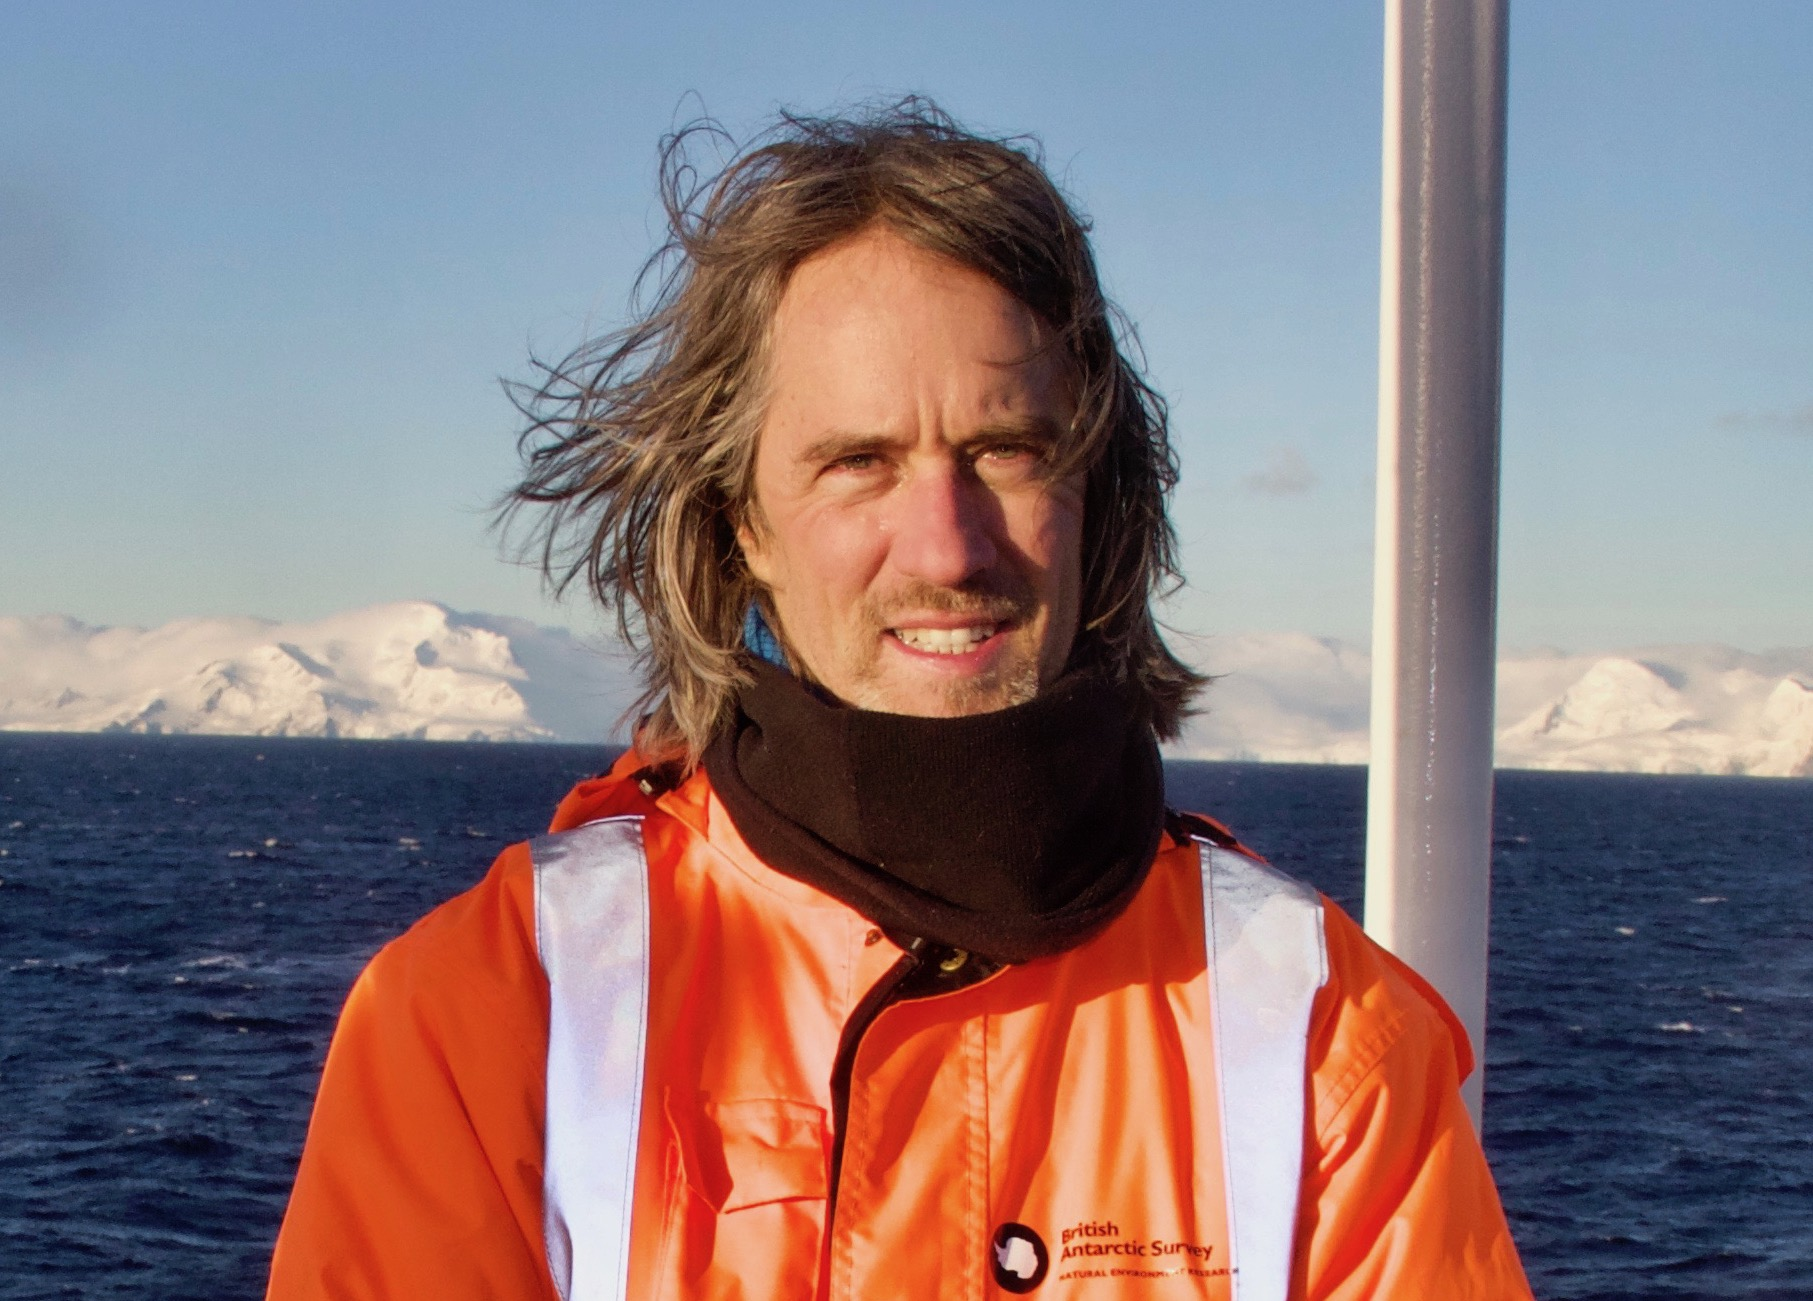
\includegraphics{Griffies_Coronation_Island_2017_crop.jpg}}
\end{center}

\textsc{\large \color{Maroon} \protect\icon{spiral.pdf} Stephen Matthew Grif\/f\/ies}
\protect\icon{ripple_spiral.pdf} 
\\[1ex]

NOAA Geophysical Fluid Dynamics Laboratory 
%$\bullet$ Princeton USA
\\
Princeton University Program in Atmospheric and Oceanic Sciences 
\\
{\tt Stephen.Griffies at noaa.gov} $\bullet$ {\tt  Stephen.M.Griffies at gmail.com} 
\\  
{\tt https://StephenGriffies.github.io/}
\\  
{\tt https://orcid.org/0000-0002-3711-236X/}

%\href{www.gfdl.noaa.gov/stephen-griffies-homepage}{research homepage} 
%$\bullet$ 
%\href{https://scholar.google.com/citations?user=4LPPPBAAAAAJ&hl=en}{google scholar page}
%\\
%Princeton USA

%\vspace{.2cm}
\end{center}
}

\section*{\sc \color{Maroon}  research statement}
\vspace{-.3cm}
My research is concerned with elements of geophysical fluid mechanics and the role of the ocean in the earth climate system. I make use of theoretical tools, idealized process models, realistic numerical circulation models, and field measurements.
Particular research topics in recent years include studies of  Atlantic and Southern Ocean dynamics; global and regional sea level variability and change;  transport of matter and energy by transient mesoscale and submesoscale eddies; subgrid scale parameterizations of turbulent ocean stirring and mixing; analysis methods aimed at revealing aspects of the ocean as a turbulent fluid; algorithms for ocean circulation models. 
I maintain active collaborations with numerous scientists from around the world, most notably in America, Australia, Europe, and India. 

\section*{\sc \color{Maroon} educational statement}
\vspace{-.3cm}
As a lecturer, mentor, author, and editor, I aim to foster a fundamental understanding of physical concepts and their creative use in describing observed and simulated ocean phenomena. Towards this aim, I strive to pedagogically articulate the foundations of geophysical fluid mechanics in articles, books, course notes, and lectures.  I am particularly interested in revealing how concepts and tools from mathematical physics can be leveraged to deepen our understanding of the ocean, and for nurturing an appreciation of geophysical fluid mechanics within the broader context of theoretical physics. 

\section*{\sc  \color{Maroon}  interests and activities}
\vspace{-.25cm}

physics, oceanography, climate, philosophy, writing, education, sustainability, cultures, meditation, yoga, surfing, skiing, walking


\section*{\sc \color{Maroon}   employment and appointments} 
\vspace{-.25cm}
\begin{tabular}{ll}

%2017--present & Partner Investigator, Australian Research Council Centre of Excellence for                              Climate Extremes \\ 

2015--present & Lecturer, , Princeton University's Atmospheric and Oceanic Sciences Program
  \\
  2013--2017  & NOAA/GFDL Model Development Team Steering Committee  \\
  Jun-Aug 2012  & Visiting Scientist, National Center for Atmospheric
                  Research, Boulder, USA \\
%  2011--2017 & Partner Investigator, Australian Research Council Centre of Excellence for                           Climate System Science \\                            
  Jan-Jun 2011   & CSIRO Distinguished Visiting Scientist Fellow, Hobart, Australia \\
  2011-present & NOAA/GFDL Senior Scientist (equivalent to university full professor) \\ 
  Mar 2009         & Visiting Professor, Universite catholique de Louvain, Belgium \\
  Jan-Nov 2005   & Visiting Scientist, CSIRO Marine and Atmospheric  Research, Hobart, Australia \\
  2001--2005     & NOAA/GFDL Oceans and Climate Group Leader \\
  2000--2011     & NOAA/GFDL Ocean Model and Climate Model Development Team (co-lead) \\
  1996-present   &  NOAA/GFDL Staff Physical Scientist \\  
  1995--1996     &  NOAA/GFDL and Princeton University Visiting Research Scientist  \\ 
  1993--1995     & UCAR Climate \& Global Change Fellow at Princeton University \\
  1988--1993     &  University of Pennsylvania Physics Graduate Research Fellow  \\                     
  1986--1987     &  Northwestern University Engineering Sciences and Applied Mathematics Fellow \\
  1984--1986     &  Louisiana State University Chemical Engineering Research Laboratory Technician                     
\end{tabular}


\section*{\sc \color{Maroon} education}
\vspace{-.25cm}
\begin{tabular}{lll}
1993-1996  &  Post-doctoral fellow in oceanography  & Princeton University \\
1988-1993  &  Ph.D in theoretical physics  & University of Pennsylvania \\
1987-1988  &  pre-PhD studies in physics & University of Washington\\
1986-1987  &  Masters in engineering sciences \& applied mathematics   & Northwestern University\\
1981-1986  &  Bachelor of science in chemical engineering  & Louisiana State University 
\end{tabular}


\section*{\sc \color{Maroon}  oceanographic field work}
\vspace{-.25cm}

%\begin{tabular}{l}
\begin{itemize}[leftmargin=*]
 \item 
 Mar-May 2017: Eight week cruise on the {\it RRS JC Ross}  to the Orkney Passage and Scotia Sea,
  as part of the
  Dynamics of the Orkney Passage Outflow (DynOPO) project. Principal Scientific Officer: A.\ Naveira Garabato. 
 \item 
  Jul 1993: Two week cruise on the {\it CCGS Hudson} to the Labrador Sea in support of  the WOCE Line AR7W Atlantic Circulation Experiment. Chief Scientist: J.\ Lazier.
\end{itemize}
%%\end{tabular}


\section*{\sc  \color{Maroon}   awards and honors}
\vspace{-.25cm}

\begin{tabular}{ll}
  2019 & Sigma Xi scientific honor society 
  \\
  2018 & Web of Sciences (Clarivate) Highly Cited Researcher 
  \\
  2017 & \href{https://eos.org/agu-news/celebrating-the-2017-class-of-fellows}{Elected Fellow of the American Geophysical Union} "For exceptional and sustained contributions to the \\ &  understanding of large-scale ocean circulation and physics and seminal advances in ocean modeling"
\\
  2017 & NOAA Administrator's Award (with Robert Hallberg) "For scientific leadership for the innovation \\ & of the versatile  community-based Modular Ocean Model MOM6" 
  \\
  2014 & \href{http://www.egu.eu/awards-medals/fridtjof-nansen/2014/stephen-m-griffies/}{European Geosciences Union Fridtjof Nansen Medal for
         Oceanographic Research}  "For 
outstanding \\ & contribution and leadership in 
ocean general circulation model development 
and critical insights in the \\ & physical 
nature and parameterization of ocean processes"
\\
  2013 & Department of Commerce Silver Medal Award (with nine other
  GFDL staff scientists): 
  "For development \\ & and application of NOAA's first comprehensive  
  Earth System Model  
  that couples the carbon cycle and \\ & climate for projection of changes" \\
  2012 & NOAA Administrator's Award "For scientific vision, leadership
  and development of 
  the Modular Ocean \\ & Model (MOM4) for climate modeling, research and
  predictions" \\
  2011 & CSIRO Distinguished Visiting Scientist Fellow, Australia \\
  2009 & Visiting Professor, Universite catholique de Louvain, Belgium\\
  2001 & NOAA/Oceanic and Atmospheric Research Outstanding Scientific
  Review Paper\\
  1999 & NOAA/Oceanic and Atmospheric Research Outstanding Scientific Paper\\
  1998 & NOAA/Oceanic and Atmospheric Research Employee of the Year\\
  1997 & NOAA/Environmental Research Laboratories Outstanding Scientific Paper\\
\end{tabular}

\section*{\sc  \color{Maroon}  professional services and memberships}
\vspace{-.25cm}

\begin{tabular}{ll}
2018-present & Editor for  \href{http://agupubs.onlinelibrary.wiley.com/hub/journal/10.1002/(ISSN)1942-2466/editorial-board/editorial-board.html}{Journal of Advances in Modeling the Earth System (JAMES)}  
\\
  2016-present & Member of the awards committee for the EGU Fridtjof Nansen Oceanography Medal 
  \\
2014-2018 &  Member  WCRP/CLIVAR Scientific Steering Group \\
2014-2016     & Co-lead of the NCEP Climate Model Development Task Force\\
2013-2018 & \href{http://www.clivar.org/clivar-panels/omdp}{WCRP/CLIVAR Ocean Model Development Panel (ex-officio)} \\
2012-2014     & CLIVAR/CliC/SCAR Southern Ocean Region Implementation Panel \\
2012-present & Emeritus member of \href{http://www.clivar.org/clivar-panels/omdp}{WCRP/CLIVAR Ocean Model Development Panel} \\
2010-present & Member European Geosciences Union \\
2009-2015     &  Scientific Advisory Board for the Catalan  Climate Institute {\it IC3}, Barcelona, Spain \\
2007-2018 & Editor of the journal Ocean Modelling \\
2006-2009     &  WCRP/CLIVAR Scientific Steering Group \\
2004-2009     &  WCRP/CLIVAR Working Group on Coupled Modelling (ex officio) \\
2004-2007     & Editorial Board of the journal {\bf Ocean Science} \\
1999-2012     & WCRP/CLIVAR Working Group on Ocean Model Development  (co-chair 2004-2009) \\
1993-present  & Member American Geophysical Union \\
1993-present  & Member American Meteorological Society \\
\end{tabular}


\section*{\sc  \color{Maroon} mentoring and sabbatical hosting}
\vspace{-.25cm}

\begin{tabular}{lll}

2019-present & Hemant Khatri & Princeton University post-doc researcher \\ 

2019     & Hussein Aluie & Princeton University visiting scholar (from University of Rochester)  \\ 

2018-present & Graeme MacGilchrist & Princeton University post-doc researcher (with Jorge Sarmiento) \\ 

2017-present & Houssam Yassin & Princeton University graduate student \\ 

2017-2018 & Laure Zanna  & Princeton University visiting scholar (from Oxford University)  \\

2017 & Jianjun Yin       & Princeton University visiting scholar (from University of Arizona)  \\

2016-2019 & Brandon Reichl       & Princeton University post-doc researcher  \\

2016-2018 & Nathaniel Tarshish & Princeton University pre-doc researcher (with Jorge Sarmiento) \\

2015-2017 & Amanda O'Rourke  & University of Michigan post-doc researcher (with Brian Arbic) \\

2015-2016    & Henri Drake             & Princeton University pre-doc researcher (with Jorge Sarmiento) \\

2014-2017 & Alison Gray            & Princeton University post-doc researcher (with Jorge Sarmiento) \\

2014-2017 & Anna FitzMaurice   & Princeton University PhD student (PhD committee) \\ 

2014-2015     & Ivy Frenger            & Princeton University post-doc researcher (with Jorge Sarmiento) \\

2013-2017 & Robert Nazarian    & Princeton University PhD student (PhD committee) \\ 

2013-2016     & Adele Morrison     & Princeton University post-doc researcher (with Jorge Sarmiento) \\

2013               & Terrence O'Kane   & Visiting senior scientist from CSIRO Marine Laboratory, Hobart, Australia \\

2012-2017     & Carolina Dufour   & Princeton University post-doc researcher (with Jorge Sarmiento)  \\

2012-2013     & Yalin Fan              & Princeton University post-doc researcher \\

2011-2014     & Michael Bueti       & University of Rhode Island  PhD student (PhD committee) \\

2008-2011     & Michael Bates       & University of New South Wales PhD student (PhD committee) \\

2005-2009     & Andreas Klocker   & University of Tasmania  PhD student (PhD committee) \\

2003-2004     & {R\"{u}diger} Gerdes  & Visiting senior scientist from AWI, Bremerhaven, Germany \\

2001-2002     & Harper Simmons   & GFDL post-doc researcher \\

1999-2002     & Shafer Smith         & Princeton University and GFDL post-doc researcher    
\end{tabular}

\section*{\sc  \color{Maroon}  university teaching}
\vspace{-.3cm}

\begin{itemize}[leftmargin=*]

\item Autumn semester 2018: Princeton University Atmospheric and Oceanic Sciences 571: Geophysical Fluid Dynamics (24 lectures covering the full course)
    
\item Spring semester 2018: Princeton University Atmospheric and Oceanic Sciences 580: Special Topics on Great Papers in Atmospheric and Oceanic Sciences (led one discussion session)

\item Autumn semester 2017: Princeton University Atmospheric and Oceanic Sciences 571: Geophysical Fluid Dynamics (24 lectures covering the full course)
  
\item Spring semester 2017: Princeton University Atmospheric and Oceanic Sciences 580: Special Topics on Great Papers in Atmospheric and Oceanic Sciences (led one discussion session)

\item Autumn semester 2016: Princeton University Atmospheric and Oceanic Sciences 571: Geophysical Fluid Dynamics (12 lectures covering the second half of the course)

\item Spring semester 2016: Princeton University Geosciences 503: Responsible Conduct of Research in Geosciences (co-taught one three-hour discussion session)

\item Autumn semester 2015: Princeton University Atmospheric and Oceanic Sciences 571: Geophysical Fluid Dynamics (12 lectures covering  the second half of the course)

\item Autumn semester 2014: Princeton University Atmospheric and Oceanic Sciences 571: Geophysical Fluid Dynamics (12 lectures covering  the first half of the course)

\item Autumn semester 1993: Princeton University Atmospheric and Oceanic Sciences 580: Data
  Assimilation in Atmospheric and Oceanic Models (co-lecturer and coordinator of visiting lectures)

\item 1990--1993:  Instructor, Undergraduate Physics Laboratory, University of Pennsylvania 

\item 1990--1993:  Teaching Assistant,  General Relativity and Quantum Field Theory, University of Pennsylvania 

\end{itemize}


\section*{\sc \color{Maroon}  participant/collaborator on research grants and projects}
\vspace{-.3cm}

\begin{itemize}[leftmargin=*]

\item Co-PI for NOAA's Climate Variability and Predictability Program Climate Process Team: Ocean Transport and Eddy Energy (2020-2022),
\$770K.

\item Co-PI for Australian Research Council Discovery Project (2019-2022): Risks of rapid ocean warming at the Antarctic continental margin. AU\$582K.

\item Co-PI for Australian Research Council Discovery Project (2019-2022): Risks of rapid ocean warming at the Antarctic continental margin. AU\$582K.

\item Co-PI for NOAA Modeling, Analysis, Predictions, and Projections Program (01Aug2018--31Jul2020): Addressing Key Issues in CMIP6-era Earth System Models. \$434K.
    
\item Program advisory board for the UK NERC funded project: Transient tracer-based Investigation of Circulation and Thermal Ocean Change (TICTOC) (2017-2020)

\item Partner Investigator for the Australian Research Council (2017-2023) Centre of Excellence for Climate Extremes, AU\$30.05M.
  
\item Co-PI for the Ocean Model Intercomparison Project (OMIP), which is part of the Coupled Model Intercomparison Project (CMIP6) (2016-present).    

\item Co-PI for the Flux Anomaly Forcing Model Intercomparison Project (FAFMIP), which is part of the Coupled Model Intercomparison Project (CMIP6) (2016-present).    

\item Co-PI for NOAA Modeling, Analysis, Predictions, and Projections Program (01Jul2016--30Jun2018): Development toward NCEP's fully-coupled global forecast and data assimilation system: A coupled wave-ocean
system.  \$316K.

\item Partner Investigator for the  Australian Research Council (2016-2020) funded project: An Australian Consortium for Eddy-Resolving Ocean-Sea Ice Modelling, AU\$599K.

\item US Department of Energy (15Aug2014--14Aug2017): Three-dimensional structure of the Southern Ocean overturning
circulation.  \$624K.

\item US National Science Foundation (01Sep2014--31Aug2020): Southern Ocean Carbon and Climate Observations and Modeling
(SOCCOM). \$20.9M

\item NASA (26Jun2014--25 Jun2017): The role of mesoscale eddies in cross-frontal transport and subduction of nutrients and carbon in
  the Southern Ocean.  \$715K.

\item NOAA (01Sept2013--31Aug2016): Signature of the Atlantic meridional overturning circulation in the North Atlantic dynamic sea
  level.  \$393K.

\item US Department of Energy (15Sep2011--14Sep2015): Mode and intermediate waters in Earth System Models. \$519K.

\item Partner Investigator for the Australian Research Council (2011-2018) Centre of Excellence for Climate System Science, AU\$21.4M.
  
\item NOAA Climate Program Office and US National Science Foundation (2010--2015): Climate Processes Team on representing internal-wave driven mixing in global ocean models.

\item NOAA Climate Program Office and US National Science Foundation (2003--2008): Climate Processes Team on ocean eddy mixed layer interactions.

\item NOAA Climate Program Office and US National Science Foundation (2003--2008): Climate Processes Team on gravity current entrainment.



\end{itemize}


\section*{\sc  \color{Maroon}  invited pedagogical lectures and special topics courses}
\vspace{-.3cm}

\begin{itemize}[leftmargin=*]

\item April/May 2019: {\sc Fundamentals of ocean models and the analysis of ocean simulations}. 15 lectures (45 minutes each) on ocean model fundamentals and analysis methods given as part of the {\bf Advanced Ocean Modelling Summer School}, Tasmania, Australia. 

\item Jan 2019: {\sc Ocean circulation
as a problem in mathematical \& computational physics:  a historical and contemporary  perspective}. Public lecture given as part of the Australian Mathematics Science Institute (AMSI) Summer School at the University of New South Wales, Sydney, Australia. 

\item Jul 2016: {\sc Ocean Modelling and sea level analysis}: three lectures (two hours each) at the International Centre for Theoretical Physics / Indian Institute for Tropical Meteorology: {\sc Advanced School on Earth System Modelling}, Pune, India

\item Aug 2013: {\sc Ocean models and ocean modeling: lectures on the fundamentals and practices}: Five lectures (two hours each) at the International Centre for Theoretical Physics School: {\sc Fundamentals of Ocean Climate Modeling at Global and Regional Scales}, Hyderabad, India

\item Mar 2009: {\sc Physical Processes Setting the Ocean's Water Masses}: four lectures (two hours each) at the Universit\'e Catholique de Louvain, Belgium

\item Nov 2007: {\sc Ocean Model Fundamentals}: 10 lectures (two hours each) at the University of Tasmania, Australia 

\item Aug 2006: {\sc Ocean Model Fundamentals}: two lectures (one hour each) at the NSF summer school, {\sc Modern Mathematical Methods in
Physical Oceanography}, Breckenridge, USA

\item Oct 2004: {\sc Ocean Model Fundamentals}: 10 lectures (two hours each) at the {\sc Indian Intensive School on Large-Scale Ocean Modelling}, Bangalore, India

\item Sep 2004: {\sc Ocean Model Fundamentals}: three lectures (two hours each) at the {\sc Global Ocean Data Assimilation Experiment  Summer School}, La Londe Les Maures, France

\item May 2003: {\sc Ocean Climate Modeling at NOAA-GFDL}: two lectures (one hour each) for a workshop on ocean modeling, Hobart, Australia

\item May 2002: {\sc Ocean Climate Modeling with MOM4}: three lectures (one hour each) for a workshop on ocean modeling, Kiel, Germany

\item Jan 2001: {\sc Ocean Dynamics and Modeling}: three lectures (two hours each) at La Escuela de Verano de Universidad de Concepci\'on, Chile

\item Mar 1999: {\sc Ocean and Climate Modeling}: two lectures (90 minutes each) at {\sc Conference on Global Climate}, Barcelona,
Spain

\end{itemize}



\section*{\sc  \color{Maroon} pedagogical media outreach}
\vspace{-.3cm}

\begin{itemize}[leftmargin=*]

\item 2016: \href{https://www.youtube.com/watch?v=gaFjlZxM7S4&feature=youtu.be}{Animation of  the ocean's role in El Ni\~{n}o} 

\item 2015:  \href{https://www.youtube.com/watch?v=8VMSF28J9H4&list=PL9poquLHLLO91iC_6pujn6bsMCvMyJ3xU}{Animation  of  Southern Ocean circulation} 

\item 2011:  \href{https://vimeo.com/27076776}{Animation  of  ocean surface temperatures from an eddying climate model} 

\end{itemize}



\section*{\sc \color{Maroon} invited research presentations since 2010}
\vspace{-.3cm}

\begin{itemize}[leftmargin=*]

\item May 2018: {\sc Understanding and projecting global, regional, and coastal sea level: Reasons to include coastal ocean processes in global models}: Consortium for Ocean-Sea Ice Modelling in Australia (COSIMA) Annual Meeting, Australian National University, Canberra, Australia \& University of New South Wales, Sydney, Australia. 

\item Mar 2018: {\sc Understanding and projecting global, regional, and coastal sea level: Reasons to include coastal ocean processes in global models}: ISSI workshop on understanding the relationship between coastal sea level and large-scale ocean circulation, Bern, Switzerland. 

\item Feb 2018: {\sc Subsurface Warming of Antarctic Coastal Waters: a Role for Both Winds and Freshening}: {\sc American Geophysical Union Ocean Sciences Conference}, Portland, Oregon, USA.

\item Dec 2017: {\sc Localized Rapid Warming of West Antarctic Subsurface Waters by Remote Winds}: American Geophysical Union Fall Meeting, New Orleans, Louisiana, USA. 

\item Nov 2017: {\sc Physical mechanisms of sea level variations in a changing climate}: International CLIVAR Scientific Steering Group meeting, Indian Institute of Tropical Meteorology, Pune, India.


\item Jul 2017: {\sc Localized rapid warming of West Antarctic
    subsurface waters by remote winds}: WCRP Conference on Regional
  Sea-level Changes and Coastal Impacts, Columbia University, New York City, USA. 

\item May 2017: {\sc Localized rapid warming of West Antarctic
    subsurface waters by remote winds}: {\it RRS JC Ross} research cruise
  JR16005 to Orkney Passage, Southern Ocean.

\item Jan 2017: {\sc The ocean mesoscale: observations, theory, and
    modeling}: Banff International Research Station (BIRS) workshop:
  {\it Transport in unsteady flows: From deterministic structures to
    stochastic models and back again}, Banff, Canada.

\item July 2016: {\sc Elements of sea level in a changing climate}:
  Indian Institute of Tropical Meteorology, Pune, India.

\item July 2016: {\sc Ocean modelling: an introduction for
    mathematical physicists}: Department of Mathematics, Savitribai
  Phule Pune University, Pune, India.

\item May 2016: {\sc Elements of sea level in a changing climate}:
  University of New South Wales, Sydney, Australia \& Australian
  National University, Canberra, Australia.

\item Jan 2016: {\sc Elements of sea level in a changing climate}:
  Louisiana State University Chemical Engineering Department, Baton
  Rouge, Louisiana, USA.

\item Oct 2015: {\sc Impacts on ocean heat from the mesoscale}:
  Lamont-Doherty Earth Observatory / Columbia University, USA.

\item Oct 2015: {\sc Impacts on ocean heat from the mesoscale}: Stony
  Brook Marine Sciences, Stony Brook, USA.

\item Oct 2014: {\sc Impacts on ocean heat from the mesoscale}:
  Meeting on ocean heat uptake at National Oceanography Centre,
  Southampton, UK.

\item Jun 2014: {\sc Impacts on ocean heat from the mesoscale}:
  University of Stockholm, Sweden.

\item Apr 2014: {\sc Problems and prospects with ocean mesoscale
    eddying climate models}: Nansen Medal lecture at the European
  Geosciences Union annual meeting, Vienna, Austria.

\item Apr 2014: {\sc Problems and prospects with ocean mesoscale
    eddying climate models}: lecture given at a CLIVAR workshop on
  eddying ocean climate models, Kiel, Germany.

\item Sep 2013: {\sc Problems and prospects of model comparisons: an
    ocean process perspective}: lecture given at a symposium
  celebrating the 80th birthday of Gerold Siedler, Kiel, Germany.

\item Feb 2013: {\sc Sea level in a suite of forced global ocean-ice
    simulations}: CLIVAR workshop on Sea-Level Rise, Ocean/Ice-Shelf
  Interactions, and Ice Sheets, Hobart, Australia

\item Jan 2013: {\sc Ocean model numerics and physics: challenges for
    mesoscale eddying global climate simulations}: 10th annual meeting
  of the Drakkar Ocean Modelling Consortia, Grenoble, France

\item Sep 2012: {\sc Sea level in ocean climate models: fundamentals
    and practices}: University of Tasmania, Hobart, Australia

\item Sep 2012: {\sc Ocean modelling with MOM and its relation to
    Australian ocean climate science}: Second meeting of Consortia for
  Ocean Modelling in Australia, Hobart, Australia

\item Feb 2012: {\sc Ocean modelling with MOM and its relation to
    Australian ocean climate science}: First meeting of Consortia for
  Ocean Modelling in Australia, Hobart, Australia

\item Mar 2011: {\sc Dynamic sea level, static sea level, and the
    non-Boussinesq steric effect}: Australia National University,
  Canberra, Australia

\item Nov 2010:  {\sc Ocean Climate Modeling at GFDL}: Scientific
  Workshop for the Centre for Australian Weather and Climate Research,
  Hobart, Australia

\item Sep 2010:  {\sc Sensitivity of Atlantic ocean variability to
    ocean physics and vertical coordinate}: CLIVAR WGOMD/GSOP Workshop
  on Decadal Variability, Predictability, and Predictions:
  Understanding the Role of the Ocean. Boulder USA 

%\item Apr 2008:  {\sc Physical Problems in Simulating the Ocean Climate System}: presentation given during a workshop on Oceans and Climate at Yale University 

%\item Mar 2008:  {\sc Physical Problems in Simulating the Ocean Climate System}: presentation given during a special session on  Climate Physics at the American Physical Society's March Meeting of Condensed Matter Physics 


\end{itemize}


\section*{\sc  \color{Maroon}  convener/organizer of workshops \& meetings}
\vspace{-.3cm}


\begin{itemize}[leftmargin=*]

\item Mar 2019: scientific advisory committee for the WCRP/CLIVAR workshop: Sources and sinks of ocean mesoscale eddy energy, Florida State University, Tallahassee, Florida, USA. 

\item Feb 2018: co-convener for the Town Hall: Process understanding and standardized assessment towards the eddying realm. {\sc American Geophysical Union Ocean Sciences Conference}, Portland, Oregon, USA.

\item Feb 2018: co-convener for the session: Modeling the Climate System at High Resolution, {\sc American Geophysical Union Ocean Sciences Conference}, Portland, Oregon, USA.

\item Sep 2016: Science Organizing Committee and Executive Planning
  Team for {\sc CLIVAR Open Science Conference}, Qingdao, China.

\item Apr 2014: {\sc Physical and biogeochemical ocean modelling: development, assessment, and applications}, Session at the European Geosciences Union General Assembly, Vienna, Austria.

\item Feb 2014: {\sc Physical and biogeochemical ocean modeling:
    development, assessment and applications}, Session at the Ocean
  Sciences meeting, Honolulu, Hawaii.

\item Apr 2013: {\sc Physical and biogeochemical ocean modelling:
  development, assessment, and applications}, Session at the European
Geosciences Union General Assembly, Vienna, Austria.

\item Feb 2013: {\sc CLIVAR WGOMD/SOP Workshop on Sea-Level Rise,
  Ocean/Ice-Shelf Interactions, and Ice Sheets}, Hobart, Australia.  

\item Apr 2012: {\sc Physical and biogeochemical ocean modelling:
  development, assessment, and applications}, Session at the European
Geosciences Union General Assembly, Vienna, Austria.

\item Oct 2011: {\sc Ocean Circulation and Ventilation}, Session at
the WCRP Open Science Conference, Denver, USA. 

\item Apr 2011: {\sc Physical and biogeochemical ocean modelling:
  development, assessment, and applications}, Session at the European
Geosciences Union General Assembly, Vienna, Austria.

\item Oct 2009: {\sc Workshop on Ocean Climate Modeling},
  GFDL/Princeton, USA.

 \item Apr 2009: {\sc CLIVAR Workshop on Ocean Mesoscale Eddies:
    Observations, Simulations, and Parameterizations}, Exeter, UK.

\item Aug 2007: {\sc CLIVAR Workshop on Numerical Methods in Ocean
  Modelling}, Bergen, Norway.

\item Nov 2005: {\sc CLIVAR Workshop on Modelling the Southern
  Ocean}, Hobart, Australia.

\item Jun 2004: {\sc CLIVAR Workshop on Evaluating the Ocean
  Component of IPCC Models}, Princeton, USA.

\item Aug 2002: {\sc Workshop on Z-coordinate Ocean Modeling},
Massachusetts Institute of Technology, USA.

\item Nov 1999: {\sc Meeting of Z-coordinate Ocean Modeling at GFDL,
  LANL, MIT, and NCAR}, Princeton, USA.

\item Jul 1999: {\sc Ocean/Atmosphere Variability and
  Predictability}, Session at the International Union of Geodesy and
Geophysics, Birmingham, UK.

\end{itemize}


\section*{\sc \color{Maroon}  student participant in competitive special topic schools}
\vspace{-.3cm}

\begin{itemize}[leftmargin=*]

\item Jan 1998: NATO Advanced Study Institute: {\sc Ocean Modeling
    and Parameterization}, Les Houches, France.

\item Jan 1996: NATO Advanced Study Institute: {\sc Climate
  Variability and Predictability}, Les Houches, France.

\item Jul 1994: Meeting of UCAR Global and Climate Change Fellows.
Steamboat Springs, USA.  

\item Jul 1992: Theoretical Advanced Study Institute: {\sc From
  String Theory to Black Holes}, Boulder, USA.

\item Jul 1991: High Energy Physics and Cosmology School, Center for
Theoretical Physics, Trieste, Italy.

\item Jun 1991: Theoretical Physics Summer School: {\sc Particle
  Physics in the 1990's}, Les Houches, France.

\end{itemize}


%\input{cv_smg_pubs_6}
\section*{\sc \color{Maroon} documents under review or in preparation}

\small 


%\begin{enumerate}[leftmargin=*]
\begin{etaremune}

\item An assessment of the Indian Ocean mean state and seasonal cycle in a suite of interannual CORE-II simulations, 2019: H. Rahaman, U. Srinivasu,  S. Panickal, J. Durgadoo, S.M. Griffies, M. Ravichandran, A. Bozec , A. Voldoire, A. Cherchi, G. Danabasoglu, H. Tsujino, K. Getzlaff, M. Ilicak, Q. Wang, R. Farneti, S. Valcke, S.J. Marsland, {\it in preparation for Ocean Modelling}.

\item ACCESS-OM2: A Global Ocean-Sea Ice Model at Three Resolutions, 2018: A.E. Kiss, A. McC.Hogg, N. Hannah, G. Brassington, F. Dias, C. Domingues, M.H. England, R. Fiedler, S.M. Grif\/f\/ies,  A. Heerdegen, P. Heil, R. Holmes, S.J. Marsland, A.K. Morrison, J. Munroe, P. Oke, M. Nikurashin, A. Savita, P. Spence, K.D. Stewart, M. Ward, F. Wu, {\it in prep for Geoscientific Model Development}.  
\item An extrema-diminishing general-coordinate implementation of neutral diffusion, 2019: A. Shao, A.J. Adcroft, R.W. Hallberg, and {\bf S.M. Grif\/f\/ies}, {\it in preparation for Journal of Advances in Modeling the Earth System (JAMES)}.

\item Relating boundary freshwater fluxes to surface salinity forcing, 2018: A.J.G. Nurser and {\bf S.M. Grif\/f\/ies}, {\it in preparation for Journal of Physical Oceanography}.

\item Towards comprehensive observing and modeling systems for monitoring and predicting regional to coastal sea level, 2018: R.M. Ponte, M. Carson, M. Cirano, C. Domingues, S. Jevrejeva, M. Marcos, G. Mitchum, R.S.W. van de Wal, P.L. Woodworth, M. Ablain, F. Ardhuin, V. Ballu, M. Becker, J. Benveniste, F. Birol, E. Bradshaw, A. Cazenave, P. De Mey-{Fr\'{e}maux}, F. Durand, T. Ezer, L.-L. Fu, I. Fukumori, K. Gordon, M. Gravelle, S.M. Grif\/f\/ies, W. Han, A. Hibbert, C.W. Hughes, D. Idier, V.H. Kourafalou, C.M. Little, A. Matthews, A. Melet, M. Merrifield, B. Meyssignac, S. Minobe, T. Penduff, N. Picot, C. Piecuch, R.D. Ray, L. Rickards, A. Santamaría-Gómez, D. Stammer, J. Staneva, L. Testut, K. Thompson, P. Thompson, S. Vignudelli, J. Williams, S.D.P. Williams, G. Wöppelmann, L. Zanna, and X. Zhang, {\it submitted to Frontiers in Marine Science} as part of OceanObs2019.


\item Ocean climate observing requirements in support of Climate Research and Climate Information, 2018: D. Stammer, A. Bracco, L. Beal, N. Bindoff, P. Braconnot, W. Cai, D. Chen, G. Danabasoglu, B. Dewitte, R. Farneti, K. Takahashi Guevara, B. Fox Kemper, J. Fyfe, S.M. Griffies, S. Jayne, R.M. Koll, A. Lazar, M. Lengaigne, X. Lin, S. Marsland, P.M.S. Monteiron, W. Robinson, R. Rykaczewski, S. Speichy, I. Smith, A. Solomon, J. Vialard, {\it submitted to Frontiers in Marine Science} as part of OceanObs2019.

\item Challenges and Prospects in Ocean Circulation Models, 2018: B. Fox-Kemper, A.J. Adcroft, C.W. {B\"{o}ning}, E.P. Chassignet, E. Curchitser, G. Danabasoglu, C. Eden, M.H. England, R. Gerdes, R. Greatbatch, S.M. Grif\/f\/ies, R.W. Hallberg, E. Hanert, P. Heimbach, H.T. Hewitt, C.N. Hill, Y. Komuro, S. Legg, J. Le Sommer, S. Masina, S.J. Marsland, S.G. Penny, F. Qiao, T.D. Ringler, A.M. Treguier, H. Tsujino, P. Uotila, S.G. Yeager,
{\it submitted to Frontiers in Marine Science} as part of OceanObs2019.

\item Sea level and the role of coastal trapped waves in mediating the interaction between the coast and open ocean, 2018: C.W. Hughes, I. Fukumori, {\bf S.M. Grif\/f\/ies}, J.M. Huthnance, S. Minobe, J.P. Spence, K.R. Thompson, and A. Wise, {\it in review at Surveys in Geophysics}.

\item Concepts and terminology for sea level--mean, variability and change, both local and global, 2019: J.M. Gregory, {\bf S.M. Grif\/f\/ies}, C.W. Hughes, J.A. Lowe, J.A. Church, I. Fukimori, 5.N. Gomez, R.E. Kopp, F. Landerer, R.M. Ponte, D. Stammer, M.E. Tamisiea, R.S.W. van de Wal, {\it in review at Surveys in Geophysics}.

\item A new algorithm to accurately calculate neutral tracer gradients and their impacts on vertical heat transport and water mass transformation, 2018: S. Groeskamp, P. Barker, T.J. McDougall, R.P. Abernathey, and {\bf S.M. Grif\/f\/ies}, {\it in review at Journal of Physical Oceanography}.

\item Rapid mixing and exchange of deep-ocean waters in an abyssal boundary current, 2018: A.C. Naveira Garabato, E.E. Frajka-Williams, C.P. Spingys, S.A. Legg, K.L. Polzin, A. Forryan, E.P. Abrahamsen, C.E. Buckingham, {\bf S.M. Grif\/f\/ies}, S.D. McPhail, K.W. Nicholls, L.F. Thomas, and M.P. Meredith,  {\it in review at Science}.

\item 100 Years of Earth System Model Development, 2018: D. Randall, C.M. Bitz, G. Danabasoglu, A.S. Denning, P. Gent, A. Gettelman, {\bf S.M. Grif\/f\/ies}, P. Lynch, H. Morrison, R. Pincus, J. Thurburn, {\it in revision for publication in A Century of Progress in Atmospheric and Related Sciences: Celebrating the American Meteorological Society Centennial}.   
       
%\item The direction of mesoscale eddy induced lateral mixing in the ocean, 2017: T.J. McDougall, {\bf S.M.} Grif\/fies, and S. Groeskamp, {\it in review at Journal of Physical Oceanography}.


%\end{enumerate}
\end{etaremune}


\section*{\sc \color{Maroon} peer-reviewed publications}

\small 

\begin{etaremune}
%\begin{enumerate}[leftmargin=*]

\item Surface winds from atmospheric reanalysis lead to contrasting oceanic forcing and coastal upwelling patterns, 2018: F.G. Taboada, C.A. Stock, {\bf S.M. Grif\/f\/ies}, J.P. Dunne, J.G. John, R.J. Small, H. Tsujino, {\it Ocean Modelling},
\\ doi:10.1016/j.ocemod.2018.11.003.

\item Understanding the Equatorial Pacific Cold Tongue Heat Budget, Part I: Diagnostic Framework, 2018: S. Ray, A.T. Wittenberg, {\bf S.M. Griffies}, and F. Zeng, {\it Journal of Climate}, {\bf 31}, 9965--9985, doi:10.1175/JCLI-D-18-0152.1. 

\item Understanding the Equatorial Pacific Cold Tongue Heat Budget, Part II: Evaluation of the GFDL-FLOR Coupled GCM, 2018: S. Ray, A.T. Wittenberg, {\bf S.M. Griffies}, and F. Zeng, {\it Journal of Climate}, {\bf 31}, 9987--10011, doi:10.1175/JCLI-D-18-0153.1.

\item Improved Simulations of Tropical Pacific Annual-Mean Climate in the GFDL FLOR and HiFLOR Coupled GCMs, 2018:  A.T. Wittenberg, G.A. Vecchi, T.L. Delworth, A. Rosati, W.G. Anderson, W.F. Cooke, S. Underwood, F. Zeng, {\bf S.M. Grif\/f\/ies}, S. Ray, {\it Journal of Advances in Modeling the Earth System (JAMES)}, doi:10.1029/2018MS001372. 


\item Science in a world of transient climate change: enabling regional to local predictions in support of reliable climate information, 2018: D. Stammer, A. Bracco, P. Bracconot, G. Brasseur, {\bf S.M. Grif\/f\/ies}, E. Hawkins, {\it Earth's Future}, \\ doi:10.1029/2018EF000979.

\item Change in future climate due to Antarctic meltwater, 2018: B. Bronselaer, M. Winton, {\bf S.M. Grif\/f\/ies}, R.J. Stouffer, W.J. Hurlin, O.V. Sergienko, K. Rodgers, J. Russell, {\it  Nature}, doi:10.1038/s41586-018-0712-z.

\item The KPP boundary layer scheme for the ocean: revisiting its formulation and benchmarking one-dimensional simulations relative to LES,  2018: L. Van Roekel, A.J.  Adcroft, G. Danabasoglu, {\bf S.M. Grif\/f\/ies}, B. Kauffman, W. Large, M. Levy, B.G. Reichl, T. Ringler, M. Schmidt, {\it Journal of Advances in Modeling the Earth System (JAMES)}, doi:10.1029/2018MS001336

\item Role of ocean model formulation in climate response uncertainty, 2019: J.P. Krasting, R.J. Stouffer, {\bf S.M. Grif\/f\/ies}, R.W. Hallberg, S.L. Malyshev, B.L. Samuels, and L.T. Sentman, {\it Journal of Climate}, {\bf 31}, 9313-9333, doi:10.1175/JCLI-D-18-0035.1.

\item The water mass transformation framework for ocean physics and biogeochemistry, 2019: S. Groeskamp, {\bf S.M. Grif\/f\/ies}, D. Iudicone,  R. Marsh, A.J.G. Nurser, and J.D. Zika, {\it Annual Review of Marine Science}, {\bf 11}, 21.1-21.35,
doi:10.1146/annurev-marine-010318-095421.


\item Roles of the ocean mesoscale in the horizontal supply of mass, heat, carbon and nutrients to the Northern Hemisphere subtropical gyres, 2018: A. Yamamoto, J.B. Palter, C.O. Dufour, {\bf S.M. Grif\/f\/ies}, C. Dianchi, M. Claret, J.P. Dunne, I. Frenger, and E.D. Galbraith, {\it Journal of Geophysical Research - Oceans},  doi:10.1029/2018JC013969.





% start of fiscal 2019 above

\item The benefits of global high-resolution for climate simulation: process-understanding and the enabling of stakeholder decisions at the regional scale, 2018: M. J. Roberts, P. L. Vidale, C. Senior, H. Hewitt, P. Chang, H. Christensen, S. Danilov, M.-E. Demory, {\bf S.M. Grif\/f\/ies}, R. Haarsma, T. Jung, S. Minobe, T. Ringler, M. Satoh, R. Schiemann, E. Scoccimarro, G. Stephens, M.F. Wehner, G. Martin, S. Bertou, C. Bates, {\it Bulletin of the American Meteorological Society}, doi:10.1175/BAMS-D-15-00320.1. 

\item Identifying Lagrangian coherent structures in a mesoscale eddy-permitting ocean model, 2018: Tarshish, N., R. Abernathey, C. Zhang, C.O. Dufour, I. Frenger, {\bf S.M. Grif\/f\/ies}, \textit{Ocean Modelling}, {\bf 130}, 15--28, doi:10.1016/j.ocemod.2018.07.001.

\item JRA-55 based surface dataset for driving ocean-sea-ice models (JRA55-do), 2018: H. Tsujino, S. Urakawaa, H. Nakano, R.J. Small, W.M. Kim, S.G. Yeager, G. Danabasoglu, T. Suzuki, J.L. Bamber, M. Bentsen, C. {B\"{o}ning}, A. Bozec, E. Chassignet, E. Curchitser, F.B. Dias, P.J. Durack, {\bf S.M. Grif\/f\/ies}, Y. Harada, M. Ilicak, S.A. Josey, C. Kobayashi, S.a Kobayashi, Y. Komuro, W.G. Large, J. {Le Sommer}, S.J. Marsland, S. Masina, M. Scheinert, H. Tomita, M. Valdivieso, D. Yamazaki, {\it Ocean Modelling},  {\bf 130}, 79-139, doi:10.1016/j.ocemod.2018.07.002.

\item Lagrangian timescales of Southern Ocean upwelling in a hierarchy of model resolutions, 2018: H.F. Drake, A.K. Morrison, {\bf  S.M. Grif\/f\/ies}, J.L. Sarmiento, W. Weijer, A. Gray, {\it  Geophysical Research Letters}, {\bf 45}, doi:10.1002/2017GL076045

\item  Lagrangian ocean analysis: fundamentals and practices, 2018: E. van Sebille, {\bf S.M. Grif\/f\/ies}, R. Abernathey, T.P. Adams, P. Berloff, A. Biastoch, B. Blanke, E.P. Chassignet, Y. Cheng, C.J. Cotter, E. Deleersnijder, K. {D\"{o}\"{o}̈s}, H. Drake, S. Drijfhout, S.F. Gary, A.W. Heemink, J. Kjellsson, I.M. Koszalka, M. Lange, C. Lique, G.A.  MacGilchrist, R. Marsh, G.C. Mayorga Adame, R. McAdam, F. Nencioli, C.B. Paris, M.D. Piggott, J.A. Polton, S. {R\"{u}hs}, S.H. Shah, M.D. Thomas, J. Wang, P.J. Wolfram, L. Zanna, and J.D. Zika, {\it Ocean Modelling},
{\bf 121}, 49--75,  doi:10.1016/j.ocemod.2017.11.008.

\item Frequency-domain analysis of forced versus intrinsic ocean surface kinetic energy variability in GFDL's CM2-O model hierarchy, 2018: A.K. O'Rourke, B.K. Arbic, and {\bf S.M. Grif\/f\/ies}, {\it Journal of Climate}, {\bf 31}, 1789--1810, doi:10.1175/JCLI-D-17-0024.1.

\item Do high-resolution global ocean models promise benefits for coupled prediction on short-range to climate timescales?, 2017: H.T. Hewitt, M.J. Bell, E.P. Chassignet, A. Czaja, D. Ferreira, {\bf S.M. Grif\/f\/ies}, P. Hyder, J. McClean, A.L. New, M.J. Roberts, {\it Ocean Modelling}, {\bf 120}, 120--136, doi:10.1016/j.ocemod.2017.11.002.

\item Multi-decadal weakening of Indian Ocean summer monsoon circulation induces an increasing northern Indian Ocean sea level, 2017: Swapna P., J. Jyoti, R. Krishnan, S. Setti, and {\bf  S.M. Grif\/f\/ies}, {\it Geophysical Research  Letters}, \newline doi:10.1002/2017GL074706.


% start of fiscal 2018 above

\item Mechanistic drivers of re-emergence of anthropogenic carbon in the Equatorial Pacific, 2017: P. Zhai, K.B. Rodgers, {\bf S.M.} Grif\/fies, R.D. Slater, D. Iudicone, J.L. Sarmiento, and L. Resplandy, {\it Geophysical Research Letters}, doi:10.1002/2017GL073758.

\item CO2-induced ocean warming around the Antarctic ice sheet in an eddying global climate model, 2017: P. Goddard, C.O. Dufour, J. Yin, {\bf S.M. Grif\/f\/ies}, M. Winton, {\it Journal of Geophysical Research}, doi:10.1002/2017JC012849. 

\item Preconditioning of the Weddell Sea polynya by the ocean mesoscale and dense water overflows, 2017: C.O. Dufour, A.K. Morrison, {\bf S.M. Grif\/f\/ies}, I. Frenger, H.M. Zanowski, M. Winton, {\it Journal of Climate}, {\bf 30}, 7719--7737, doi:10.1175/JCLI-D-16-0586.1

\item Spiraling pathways of global deep waters to the surface of the Southern Ocean, 2017: V. Tamsitt, H.  Drake, A.K. Morrison, L.D. Talley, C.O. Dufour, A.R. Gray, {\bf S.M. Grif\/f\/ies}, M.R. Mazloff, J.L. Sarmiento, J. Wang, and W. Weijer, {\it Nature Communication}, doi:10.1038/s41467-017-00197-0.

\item Localized rapid warming of West Antarctic Peninsula subsurface waters by remote winds, 2017: P.J. Spence, R. Holmes, A. McC. Hogg,   {\bf S.M. Grif\/f\/ies}, K.D. Stewart, and M.H. England, {\it Nature Climate Change}, doi:10.1038/NCLIMATE3335.

\item Biogeochemical protocols and diagnostics for the CMIP6 Ocean Model Intercomparison Project (OMIP), 2017: J.C. Orr, R.G. Najjar, O. Aumont, L.  Bopp, J. Bullister, G. Danabasoglu, S. Doney,  J.P. Dunne, J.-C. Dutay, H. Graven, {\bf S.M. Grif\/f\/ies}, J.G. John, F. Joos, I. Levin, K. Lindsay, R. J. Matear, A. Mouchet, G. McKinley, A. Oschlies, A. Romanou, R. Schlitzer, A. Tagliabue, T. Tanhua, and A. Yool, {\it Geoscientific Model Development}, {\bf 10}, 2169--2199, doi:10.5194/gmd-10-2169-2017.

\item Climate Process Team on Internal-Wave Driven Ocean Mixing, 2017:  J.A. MacKinnon,
Z. Zhao, C.B. Whalen, A.F. Waterhouse, D.S. Trossman, O.M. Sun, L.C. St. Laurent, H.L. Simmons, K. Polzin, R. Pinkel, A. Pickering, 
N.J. Norton, J.D. Nash, R. Musgrave, L.M. Merchant, A.V. Melet, B. Mater, S. Legg, 
W.G. Large, E. Kunze, J.M. Klymak,  M. Jochum, S.R. Jayne, R.W. Hallberg, {\bf S.M. Grif\/f\/ies}, P. Gent, S. Diggs, G. Danabasoglu, E.P. Chassignet, M.C. Buijsman, 
 F.O. Bryan, B.P. Briegleb, A. Barna, B.K. Arbic,  J.K. Ansong, M.H. Alford, {\it Bulletin of the American Meteorological Society}, doi:10.1175/BAMS-D-16-0030.1.

\item Vertical resolution of baroclinic modes in global ocean models,
  2017: K. Stewart, A. McC Hogg, S.M. Grif\/f\/ies, A.P. Heerdegen,
  M.L. Ward, P.J. Spence, M.H. England,  {\it Ocean Modelling},
  {\bf 113}, 50--65, doi:10.1016/j.ocemod.2017.03.012.

\item The Flux-Anomaly-Forced Model Intercomparison Project (FAFMIP)
  for investigation of sea-level and ocean climate change in response
  to CO2 forcing, 2016: J. Gregory, N. Bouttes-Mauhourat, {\bf
    S.M. Grif\/f\/ies}, H. Haak, W.J. Hurlin, J.  Jungclaus,
  M. Kelley, W.G. Lee, J. Marshall, A. Romanou, O.A. Saenko,
  D. Stammer, and M.  Winton, {\it Geoscientific Model Development},
  {\bf 9}, 3993--4017, doi:10.5194/gmd-9-3993-2016.





% start of fiscal 2017 above

\item OMIP contribution to CMIP6: experimental and diagnostic protocol for the physical component of the Ocean Model Intercomparison  Project, 2016: {\bf S.M. Grif\/f\/ies}, G. Danabasoglu, P.J. Durack,
  A.J. Adcroft, V. Balaji, C. B\"{o}̈ning, E.P. Chassignet,
  E. Curchitser, J. Deshayes, H. Drange, B. Fox-Kemper, P.J. Gleckler,
  J.M. Gregory, H. Haak, R.W. Hallberg, P. Heimbach, H.T. Hewitt,
  D.M. Holland, T. Ilyina, J.H. Jungclaus, Y. Komuro, J.P. Krasting,
  W.G. Large, S.J. Marsland, S. Masina, T.J. McDougall, A.J.G. Nurser,
  J.C. Orr, A. Pirani, F. Qiao, R.J. Stouffer, K.E. Taylor,
  A.M. Treguir, H. Tsujino, P. Uotila, M. Valdivieso, Q. Wang,
  M. Winton, and S.G. Yeager, {\it Geoscientific Model Development},
  {\bf 9}, 3231--3296, doi:10.5194/gmd-9-3231-2016.

\item North and Equatorial Pacific Ocean Circulation in the CORE-II
  Hindcast Simulations, 2016: Y. Tseng, H.Lin, H. Chen, K.  Thompson,
  M. Bentsen, C. B\"{o}ning, A. Bozec, C. Cassou, E.  Chassignet,
  C. Chow, G. Danabasoglu, S. Danilov, R. Farneti, Y. Fujii, {\bf
    S.M. Grif\/f\/ies}, M. Ilicak, T. Jung, S. Masina, A. Navarra,
  L. Patara, B.L.  Samuels, M. Scheinert, D. Sidorenko, C. Sui,
  H. Tsujino, S. Valcke, A. Voldoire, Q. Wang, {\it Ocean Modelling},
  {\bf 104}, 143--160, doi:10.1016/j.ocemod.2016.06.003.

\item The influence of geothermal heating on Southern Ocean
  circulation in a global climate model, 2016: S.M. Downes,
  A. McC. Hogg, {\bf S.M. Grif\/f\/ies}, and B.L. Samuels, {\it
    Journal of Climate}, {\bf 29}, 5689--5708,
  doi:10.1175/JCLI-D-15-0458.1.

\item Mechanisms of Southern Ocean heat uptake and transport in a
  global eddying climate model, 2016: A.K. Morrison, {\bf
    S.M. Grif\/f\/ies}, M. Winton, W.G. Anderson, and J.L. Sarmiento,
  {\it Journal of Climate}, {\bf 29}, 2059--2075,
  doi:10.1175/JCLI-D-15-0579.1

\item An assessment of the Arctic Ocean in a suite of interannual
  CORE-II simulations. Part III: Hydrography and fluxes, 2016:
  M. Ilicak, H. Drange, Q. Wang, R. Gerdes, Y. Aksenov, D. Bailey,
  M. Bentsen, A. Biastoch, A. Bozec, C. B\"{o}ning, C. Cassou,
  E. Chassignet, A.C. Coward, B. Curry, G. Danabasoglu, S. Danilov,
  E. Fernandez, P.G. Fogli, Y. Fuji, {\bf S.M. Grif\/f\/ies},
  D. Iovino, A. Jahn, T. Jung, W.G. Large, C. Lee, C. Lique, J. Lu,
  S. Masina, A. J.G. Nurser, C. Roth, D. Salas y M\'{e}lia,
  B.L. Samuels, P. Spence, H. Tsujino, S. Valcke, A. Voldoire,
  X. Wang, S.G. Yeager, {\it Ocean Modelling}, {\bf 100}, 141--161,
  doi:10.1016/j.ocemod.2016.02.004.

\item An assessment of the Arctic Ocean in a suite of interannual
  CORE-II simulations. Part II: liquid freshwater, 2016: Q. Wang,
  M. Ilicak, R. Gerdes, H. Drange, Y. Aksenov, D. Bailey, M. Bentsen,
  A. Biastoch, A. Bozec, C. B\"{o}ning, C.  Cassou, E. Chassignet,
  A.C. Coward, B. Curry, G. Danabasoglu, S. Danilov, E. Fernandez,
  P. Giuseppe Fogli, Y. Fujii, {\bf S.M. Grif\/f\/ies}, R. Ingvaldsen,
  D. Iovino, A. Jahn, T. Jung, W.G. Large, C. Lee, C. Lique, J. Lu,
  S. Masina, A.J.G. Nurser, B. Rabe, C. Roth, D. Salas y M\'elia,
  B.L. Samuels, P. Spence, H. Tsujino, S. Valcke, A. Voldoire,
  X. Wang, S.G. Yeager, {\it Ocean Modelling}, {\bf 99}, 86--109.

\item An assessment of the Arctic Ocean in a suite of interannual
  CORE-II simulations. Part I: Sea ice and solid freshwater, 2016:
  Q. Wang, M. Ilicak, R. Gerdes, H. Drange, Y. Aksenov, D. Bailey,
  M. Bentsen, A. Biastoch, A. Bozec, C. B\"{o}ning, C.  Cassou,
  E. Chassignet, A.C. Coward, B. Curry, G. Danabasoglu, S. Danilov,
  E. Fernandez, P. Giuseppe Fogli, Y. Fujii, {\bf S.M. Grif\/f\/ies},
  R. Ingvaldsen, D. Iovino, A. Jahn, T. Jung, W.G. Large, C. Lee,
  C. Lique, J. Lu, S. Masina, A.J.G. Nurser, B. Rabe, C. Roth,
  D. Salas y M\'elia, B.L. Samuels, P. Spence, H. Tsujino, S. Valcke,
  A. Voldoire, X. Wang, S.G. Yeager, {\it Ocean Modelling}, {\bf 99},
  110-132, doi:10.1016/j.ocemod.2015.12.008.

\item Enhanced warming of the Northwest Atlantic Ocean under climate
  change, 2016: V. S. Saba, {\bf S.M. Grif\/f\/ies}, W.G. Anderson,
  M. Winton, M.A. Alexander, T.L. Delworth, J.A. Hare, M.J. Harrison,
  A. Rosati, G.A. Vecchi, and R. Zhang, {\it Journal of Geophysical
    Research - Oceans}, doi:10.1002/2015JC011346.

\item North Atlantic Simulations in Coordinated Ocean-ice Reference
  Experiments phase II (CORE-II). Part II: Inter-Annual to Decadal
  Variability, 2016: G. Danabasoglu, S.G. Yeager, W.M. Kim,
  E. Behrens, M. Bentsen, D. Bi, A. Biastoch, R. Bleck, C. B\"{o}ning,
  A. Bozec, V.M. Canuto, C. Cassou, E. Chassignet, A.C. Coward,
  S. Danilov, N. Diansky, H. Drange, R. Farneti, E. Fernandez,
  P.G. Fogli, G. Forget, Y. Fujii, {\bf S.M. Grif\/f\/ies}, A. Gusev,
  P. Heimbach, A. Howard, T. Jung, M. Kelley, W.G. Large,
  A. Leboissetier, J. Lu, G. Madec, S.J. Marsland, S. Masina,
  A. Navarra, A. J.G. Nurser, A. Pirani, A. Romanou, D. Salas y Melia,
  B.L. Samuels, M. Scheinert, D. Sidorenko, S. Sun, A.-M. Treguier,
  H. Tsujino, P. Uotila, S. Valcke, A. Voldoire, and Q. Wang, {\it Ocean Modelling}, {\bf 97}, 65--90, 
doi:10.1016/j.ocemod.2015.11.007.

\item Atlantic multi-decadal oscillation covaries with Agulhas leakage, 2015: A. Biastoch, J.V. Durgadoo, A.K. Morrison, E. van Sebille, W. Weijer, and {\bf S.M. Grif\/f\/ies}, {\it Nature Communication}, {\bf 6}, 10082, doi:10.1038/ncomms10082.

\item Role of mesoscale eddies in cross-frontal transport of heat and biogeochemical tracers in the Southern Ocean, 2015: C.O. Dufour,
  {\bf S.M. Grif\/f\/ies}, G.F. de Souza, I. Frenger, A.K. Morrison,
  J.B. Palter, J.L. Sarmiento, E.D. Galbraith, J.P. Dunne,
  W.G. Anderson, and R.D. Slater, {\it Journal of Physical
    Oceanography}, {\bf 45}, 3057--3081. 
    doi:10.1175/JPO-D-14-0240.1.

\item An assessment of Southern Ocean water masses and sea ice during
  1988--2007 in a suite of inter-annual CORE-II simulations, 2015:
  S.M. Downes, R. Farneti, P. Uotila, {\bf S.M. Grif\/f\/ies},
  S. Marsland, D. Bailey, E. Behrens, M. Bentsen, D. Bi, A. Biastoch,
  C. B\"oning, A. Bozec, V.M. Canuto, E. Chassignet, G. Danabasoglu,
  S. Danilov, N. Diansky, H. Drange, P. Giuseppe Foglio, A. Gusev,
  A. Howard, M. Ilicak, T.  Jung, M. Kelley, W.G. Large,
  A. Leboissetier, M. Long, J. Lu, S. Masina, A. Mishra, A. Navarra,
  A.J.G. Nurser, L. Patara, B.L. Samuels, D. Sidorenko, P. Spence,
  H. Tsujino, Q. Wang, S.G. Yeager, {\it Ocean Modelling}, {\bf 94},
  67--94.  doi:10.1016/j.ocemod.2015.07.022.


% start of fiscal 2016 above this one    

\item An assessment of Antarctic Circumpolar Current and Southern
  Ocean Meridional Overturning Circulation sensitivity during
  1958--2007 in a suite of inter-annual CORE-II simulations, 2015:
  R. Farneti, S. Downes, {\bf S.M. Grif\/f\/ies}, S. Marsland,
  D. Bailey D. Bailey, E. Behrens, M. Bentsen, D. Bi, A. Biastoch,
  C. B\"oning, A. Bozec, V.M. Canuto, E. Chassignet, G. Danabasoglu,
  S. Danilov, N. Diansky, H. Drange, P. Giuseppe Foglio, A. Gusev,
  A. Howard, M. Ilicak, T.  Jung, M. Kelley, W.G. Large,
  A. Leboissetier, M. Long, J. Lu, S. Masina, A. Mishra, A. Navarra,
  A.J.G. Nurser, L. Patara, B.L. Samuels, D. Sidorenko, P. Spence,
  H. Tsujino, Q. Wang, S.G. Yeager, {\it Ocean Modelling}, {\bf 93},
  84--120. doi:10.1016/j.ocemod.2015.07.009.

\item Simulated South Atlantic transports and their variability during
  1958-2007, 2015: L.E.  Sitz, R. Farneti, {\bf S.M. Grif\/f\/ies},
  {\it Ocean Modelling}, {\bf 91}, 70--90,
  doi:10.1016/j.ocemod.2015.05.001.

\item Sensitivity of abyssal watermasses to overflow
  parameterizations, 2015, K. Snow, A. McC. Hogg, S.M. Downes,
  B.M. Sloyan, M.L. Bates, and {\bf S.M. Grif\/f\/ies}, {\it Ocean
    Modelling}, {\bf 89}, 84--103,
  doi:10.1016/j.ocemod.2015.03.004.

\item An extreme event of sea level rise along the northeast coast of
  North America in 2009-2010, 2015: P.  Goddard, J. Yin, {\bf
    S.M. Grif\/f\/ies}, and S. Zhang, {\it Nature Communication}, doi:10.1038/ncomms7346.

\item Impacts on ocean heat from transient mesoscale eddies in a
  hierarchy of climate models, 2015: {\bf S.M. Grif\/f\/ies},
  M. Winton, W.G. Anderson, R. Benson, T.L. Delworth, C.O. Dufour,
  J.P. Dunne, P. Goddard, A.K. Morrison, A. Rosati, A.T. Wittenberg,
  J. Yin, and R. Zhang, {\it Journal of Climate}, {\bf 28}, 952-977,
  doi:10.1175/JCLI-D-14-00353.1.

\item Has coarse ocean resolution biased simulations of transient
  climate sensitivity?, 2014: M.  Winton, W.G. Anderson,
  T.L. Delworth, {\bf S.M. Grif\/f\/ies}, W.J. Hurlin and A. Rosati,
  {\it Geophysical Research Letters}, doi:10.1002/2014GL061523.

\item Tropical cyclone-induced thermocline warming and its regional
  and global impacts, 2014: M.R. Bueti, I. Ginis, L.M. Rothstein, and
  {\bf S.M. Grif\/f\/ies}, {\it Journal of Climate}, {\bf 27},
  6978--6999, doi:10.1175/JCLI-D-14-00152.1.

\item On the subtropical Pacific meridional overturning circulation
  variability over the second half of the 20th century, 2014:
  R. Farneti, S. Dwivedi, F. Kucharski, F. Molteni, and {\bf
    S.M. Grif\/f\/ies}, {\it Journal of Climate}, {\bf 27},
  7102--7112.  doi:10.1175/JCLI-D-13-00707.1.

\item On geometrical aspects of interior ocean mixing, 2014:
  T.J. McDougall, S. Groeskamp, and {\bf S.M. Grif\/f\/ies}, {\it
    Journal of Physical Oceanography}, {\bf 44}, 2164--2175,
  doi:10.1175/JPO-D-13-0270.1.

\item Rapid subsurface warming and circulation changes of Antarctic
  coastal waters by poleward shifting winds, 2014: P. Spence, {\bf
    S.M. Grif\/f\/ies}, M.H. England, A. McC. Hogg, O.A. Saenko, and
  N.C. Jourdain, {\it Geophysical Research Letters}, {\bf 41},
  4601--4610, doi:10.1002/2014GL060613.

\item An assessment of global and regional sea level in a suite of
  interannual CORE-II simulations, 2014: {\bf S.M. Grif\/f\/ies},
  J. Yin, P.J. Durack, P. Goddard, S.C. Bates, E. Behrens, M. Bentsen,
  D. Bi, A. Biastoch, C. B\"oning, A. Bozec, C. Cassou, E. Chassignet,
  G. Danabasoglu, S. Danilov, C. Domingues, H. Drange, R. Farneti,
  E. Fernandez, R. J. Greatbatch, D.M. Holland, M. Ilicak, J. Lua,
  S.J. Marsland, A. Mishra, K. Lorgacher, A.J.G. Nurser, D Salas y
  M\`elia, J.B.  Palter, B.L. Samuels, J. Schr\"oter, F.U. Schwarzkopf, D. Sidorenko, A.-M. Treguier, Y. Tseng,
  H. Tsujino, P. Uotila, S. Valcke, A. Voldoire, Q. Wang, M. Winton,
  and X. Zhang, {\it Ocean Modelling}, {\bf 78}, 35--89,
  doi:10.1016/j.ocemod.2014.03.004.

\item Impacts of parameterized Langmuir turbulence and non-breaking
  wave mixing in global climate simulations, 2014: Y. Fan and {\bf
    S.M. Grif\/f\/ies}, {\it Journal of Climate}, {\bf 27},
  4752--4775, doi:10.1175/JCLI-D-13-00583.1.

\item Simulated global swell and wind sea climate and their responses
  to anthropogenic climate change at the end of the 21st century,
  2014: Y. Fan, S.-J. Lin, {\bf S.M. Grif\/f\/ies}, and M.A. Hemer,
  {\it Journal of Climate}, {\bf 27}, 3516--3536,
  doi:10.1175/JCLI-D-13-00198.1.

\item Development of a regional model for the north Indian Ocean,
  2014: H. Rahaman. M. Harrison, D. Sengupta, M.  Ravichandran, and
  {\bf S.M. Grif\/f\/ies}, {\bf 75}, 1--19, {\it Ocean Modelling},
  doi:10.1016/j.ocemod.2013.12.005.

\item North Atlantic Simulations in Coordinated Ocean-ice Reference
  Experiments phase II (CORE-II). Part I: Mean States, 2013: G.
  Danabasoglu, S. Yeager, D. Bailey, E. Behrens, M. Bentsen, D. Bi,
  A. Biastoch, C. {B\"{o}ning}, A. Bozec, V.M. Canuto, C. Cassou,
  E. Chassignet, C. Coward, S. Danilov, N. Diansky, H. Drange,
  R. Farneti, E. Fernandez , P. G. Fogli, G. Forget, Y. Fujii, {\bf
    S.M. Grif\/f\/ies}, A.  Gusev, P. Heimbach, A.  Howard, T. Jung,
  M. Kelley, W.G. Large, A. Leboissetier, J. Lu, G. Madec,
  S.J. Marsland, S. Masina, A. Navarra, A.J.G. Nurser, A. Pirani,
  D. Salas y {M\'{e}lia}, B.L. Samuels, M. Scheinert, D. Sidorenko,
  A.-M. Treguier, H. Tsujino, P.   Uotila, S. Valcke , A. Voldoire, and
  Q. Wang, {\it Ocean Modelling}, doi:10.1016/j.ocemod.2013.10.005.

\item The deep ocean buoyancy budget and its temporal variability,
  2013: J.B. Palter, {\bf S.M. Grif\/f\/ies}, E.D. Galbraith,
  A. Gnanadesikan, B.L. Samuels, and A. Klocker, {\it Journal of
    Climate}, {\bf 27}, 551--573,
  doi:10.1175/JCLI-D-13-00016.1.

\item Sea level changes forced by Southern Ocean winds, 2013:
  L.M. Frankcombe, P. Spence, A. McC. Hogg, M.H. England, and {\bf
    S.M. Grif\/f\/ies}, {\it Geophysical Research Letters}, {\bf 40},
  doi:10.1002/2013GL058104.

\item Challenges to Understanding the Dynamic Response of Greenland's
  Marine Terminating Glaciers to Oceanic and Atmospheric Forcing,
  2012: F. Straneo, P. Heimbach, O. Sergienko, G. Hamilton,
  G. Catania, {\bf S.M. Grif\/f\/ies}, R. W. Hallberg, A. Jenkins,
  I. Joughin, R. Motyka, W. T. Pfeffer, S. F. Price, E. Rignot,
  T. Scambos, M. Truffer, A. Vieli, {\it Bulletin of the American
    Meteorological Society}, {\bf 94}, 1131--1144.

\item The ACCESS coupled model: description, control climate and
  evaluation, 2013: D. Bi, M. Dix, S.J. Marsland, S. O'Farrell,
  H. Rashid, P. Uotila, A.C. Hirst, E. Kowalczyk, M. Golebiewski,
  A. Sullivan, H. Yan, N. Hanna, C. Franklin, Z. Sun, P. Vohralik,
  I. Watterson, X. Zhou, R. Fiedler, M. Collier, Y. Ma, J. Noonan,
  L. Stevens, P. Uhe, H. Zhu, {\bf S.M. Grif\/f\/ies}, R. Hill,
  C. Harris, and K. Puri, {\it Australian Meteorological and
    Oceanographic Journal}, {\bf 63}, 41--64.

\item Evaluation of ACCESS climate model ocean metrics in CMIP5
  simulations, 2013: S.J. Marsland, D. Bi, P. Uotila, R. Fiedler, {\bf
    S.M. Grif\/f\/ies}, K. Lorbacher, S. O'Farrell, A. Sullivan,
  P. Uhe, X. Zhou, and A.C. Hirst, {\it Australian Meteorological and
    Oceanographic Journal}, {\bf 63}, 101-119.

\item ACCESS-OM: the ocean and sea ice core of the ACCESS coupled
  model, 2013: D. Bi, S.J. Marsland, P. Uotila, S. O'Farrell,
  R. Fiedler, A. Sullivan, {\bf S.M. Grif\/f\/ies}, X. Zhou, and
  A.C. Hirst, {\it Australian Meteorological and Oceanographic
    Journal}, {\bf 63}, 213--232.

\item GFDL’s ESM2 global coupled climate-carbon Earth System Models
  Part II: Carbon system formulation and baseline simulation
  characteristics, 2013: J.P. Dunne, J.G. John, E.N. Shevliakova,
  R.J. Stouffer, J.P. Krasting, S.L. Malyshev, P.C.D. Milly,
  L.A. Sentman, A.J. Adcroft, W. Cooke, K.A. Dunne, {\bf
    S.M. Griffies}, R.W. Hallberg, , M.J. Harrison, H. Levy,
  A.T. Wittenberg, P.J. Phillipps, N. Zadeh, {\it Journal of Climate},
  {\bf 26}, 2247--2267, doi: 10.1175/JCLI-D-12-00150.1.

\item Influence of ocean and atmosphere components on simulated
  climate sensitivities, 2013: M. Winton, A.J. Adcroft, {\bf
    S.M. Grif\/f\/ies}, R.W. Hallberg, L.W. Horowitz and
  R.J. Stouffer, {\it Journal of Climate}, {\bf 26}, 231--245,
  doi:10.1175/JCLI-D-12-00121.1.

\item Northern high latitude heat budget decomposition and transient
  warming, 2013: M.A.A. Rugenstein, M. Winton, R.J. Stouffer, {\bf
    S.M. Griffies}, and R.W. Hallberg, {\it Journal of Climate}, {\bf 26}, 609-621, doi:10.1175/JCLI-D-11-00695.1.

\item Connecting changing ocean circulation with changing climate,
  2012: M. Winton, {\bf S.M. Grif\/f\/ies}, B.L. Samuels,
  J.L. Sarmiento, and T.L. Froelicher, {\it Journal of Climate}, {\bf 26}, 2268--2278, doi:10.1175/JCLI-D-12-00296.1.

\item GFDL’s ESM2 global coupled climate-carbon Earth System Models
  Part I: Physical formulation and baseline simulation
  characteristics, 2012: J.P. Dunne, J.G. John, A.J. Adcroft, {\bf
    S.M. Griffies}, R.W. Hallberg, E.N. Shevliakova, R.J. Stouffer,
  W. Cooke, K.A. Dunne, M.J. Harrison, J.P. Krasting, S.L. Malyshev,
  P.C.D. Milly, P.J. Phillipps, L.A. Sentman, B.L. Samuels,
  M.J. Spelman, M. Winton, A.T. Wittenberg, N. Zadeh, {\it Journal of
    Climate}, {\bf 25}, 6646--6665,
doi:10.1175/JCLI-D-11-00560.1.

\item The catalytic role of beta effect in barotropization processes,
  2012: A. Venaille, G.K. Vallis, and {\bf S.M. Griffies}, {\it
    Journal of Fluid Mechanics}, {\bf 709}, 490-515,
  doi:10.1017/jfm.2012.344.

\item A dynamic, embedded Lagrangian model for ocean climate models,
  Part II: Idealised overflow tests, 2012: M.L. Bates, {\bf
    S.M. Grif\/f\/ies}, and M.H. England, {\it Ocean Modelling}, {\bf
    59-60}, 60--76, doi:10.1016/j.ocemod.2012.08.003.

\item A dynamic, embedded Lagrangian model for ocean climate models,
  Part I: Theory and implementation, 2012: M.L. Bates, {\bf
    S.M. Grif\/f\/ies}, and M.H. England, {\it Ocean Modelling}, {\bf
    59-60}, 41--59, doi:10.1016/j.ocemod.2012.05.004.

\item Rapid barotropic sea level rise from simulated ice-sheet melting
  scenarios, 2012: K. Lorbacher, S. J. Marsland, J. A. Church, {\bf
    S.M. Griffies}, and D. Stammer, {\it Journal of Geophysical
    Research}, {\bf 117, C06003}, doi:10.1029/2011JC007733.

\item Physical processes that impact the evolution of global mean sea
  level in ocean climate models, 2012: {\bf S.M. Griffies} and R. J.\
  Greatbatch, {\it Ocean Modelling}, {\bf 51}, 37--72,
  doi:10.1016/j.ocemod.2012.04.003.

\item Impact of climate warming on upper layer of the Bering Sea,
  2012: H.-C. Lee, T.L. Delworth, A. Rosati, R. Zhang, W.G. Anderson,
  F. Zeng, C.A. Stock, A. Gnanadesikan, K.W. Dixon, {\bf
    S.M. Griffies}, {\it Climate Dynamics}, {\bf 40}, 327–340,
  doi:10.1007/s00382-012-1301-8.

\item Simulated climate and climate change in the GFDL CM2.5
  high-resolution coupled climate model, 2012: T.L. Delworth,
  A. Rosati, W. Anderson, A.J. Adcroft, V. Balaji, R. Benson,
  K. Dixon, {\bf S.M. Griffies}, H.-C. Lee, R.C. Pacanowski,
  G.A. Vecchi, A.T. Wittenberg, F. Zeng, and R. Zhang, {\it Journal of
    Climate}, {\bf 25}, 2755--2781, doi:10.1175/JCLI-D-11-00316.1.

\item Spurious dianeutral mixing and the role of momentum dissipation,
  2012: M. Ilicak, A. J. Adcroft, {\bf S.M. Griffies}, and
  R. W. Hallberg, {\it Ocean Modelling}, {\bf 45-46}, 37--58,
  doi:10.1016/j.ocemod.2011.10.003.

\item Different magnitudes of projected subsurface ocean warming
  around Greenland and Antarctica, 2011: J. Yin, J.T. Overpeck, {\bf
    S.M. Griffies}, A. Hu, J.L. Russell, and R.J. Stouffer, {\it
    Nature Geosciences}, doi:10.1038/NGEO1189.

\item Water mass exchange in the Southern Ocean in coupled climate
  models, 2011: S.M. Downes, A. Gnanadesikan, {\bf S.M. Grif\/f\/ies},
  and J.L. Sarmiento, {\it Journal of Physical Oceanography}, {\bf
    41}, 1756--1771.  doi:10.1175/2011JPO4586.1.

\item The impact of decadal-centennial climate variability on the
  distribution of radiocarbon in CM2Mc, a new earth system model,
  2011: E. Galbraith, E.Y. Hwon, A. Gnanadesikan, {\bf
    S.M. Grif\/f\/ies}, J. Dunne, K. Rodgers, J.L. Sarmiento, D.
  Bianchi, J. Simeon, A. Wittenberg, I.M. Held, and R.  Slater, {\it
    Journal of Climate}, {\bf 24}, 4230--4254.
  doi:10.1175/2011JCLI3919.1.

\item GFDL's CM3 Coupled Climate Model: Characteristics of the Ocean
  and Sea Ice Simulations, 2011: {\bf S.M. Grif\/f\/ies}, M. Winton,
  L.J. Donner, L.W. Horowitz, S.M. Downes, R.  Farneti,
  A. Gnanadesikan, W.J. Hurlin, H.-C. Lee, Z. Liang, J.B. Palter,
  B.L. Samuels, A.T. Wittenberg, B.L. Wyman, J.  Yin, and N.T. Zadeh,
  {\it Journal of Climate}, {\bf 24}, 3520--3544.  doi:
  10.1175/2011JCLI3964.1.

\item The Dynamical Core, Physical Parameterizations, and Basic Simulation Characteristics of the Atmospheric Component of the GFDL Global Coupled Model CM3, 2011: L.J. Donner, B.L. Wyman, R.S. Hemler, L.W. Horowitz,, Y. Ming, M. Zhao, J.-C. Golaz, J. Austin, W.F. Cooke, S.R. Freidenreich, P. Ginoux, C.T. Gordon, {\bf S.M. Grif\/f\/ies}, I.M. Held, W.J. Hurlin, S.A. Klein, A.R. Langenhorst, H.-C. Lee, S.-J. Lin, S. L. Maleyshev, P.C.D. Milly, R. Pincus, J.J. Ploshay, V. Ramaswamy, M.D. Schwarzkopf, C.J. Seman, E. Shevliakova, W.F. Stern, R.J. Stouffer, R. John Wilson, M.  Winton, and A.T. Wittenberg, {\it Journal of Climate}, {\bf 24}, 3484--3519. 
  doi:10.1175/2011JCLI3955.1.

\item Realistic test cases for limited area ocean modelling, 2011: M. Herzfeld, M. Schmidt, {\bf S.M. Grif\/f\/ies}, and Z. Liang, {\it    Ocean Modelling}, {\bf 37}, 1--34, doi:10.1016/j.ocemod.2010.12.008.

\item Parameterization of mixed layer eddies. III: Implementation and impact in global ocean climate simulations, 2011: B. Fox-Kemper,
  G. Danabasoglu, R. Ferrari, {\bf S.M. Grif\/f\/ies}, R.W. Hallberg, M.M. Holland, M.E. Maltrud, S. Peacock, and B.L. Samuels, {\it Ocean Modelling}, doi:10.1016/j.ocemod.2010.09.002.

\item The impact of Greenland melt on regional sea level: a preliminary comparison of dynamic and static equilibrium effects, 2010: R.E.\ Kopp, J.X.\ Mitrovica, {\bf S.M.\ Grif\/f\/ies}, C.C.\  Hay, J.\ Yin, and R.J.\ Stouffer, {\it Climatic Change Letter}.\,
  {\bf 103}, 619--625, doi:10.1007/s10584-010-9935-1.

\item The role of mesoscale eddies in the rectification of the Southern Ocean response to climate change, 2010: R.\ Farneti, T.D.\
  Delworth, A.J.\ Rosati, {\bf S.M.\ Grif\/f\/ies}, and F.\ Zeng, {\it Journal of Physical Oceanography}, {\bf 40}, 1539--1557.

\item Spatial Variability of Sea-Level Rise in 21st Century Projections, 2010: J.\ Yin, {\bf S.M.\ Grif\/f\/ies}, and R.J.\ Stouffer, {\it Journal of Climate}, {\bf 23}, 4585-–4607,
doi:10.1175/2010JCLI3533.1.

\item Boundary-value problem for the parameterized mesoscale eddy transport, 2010: R.\ Ferrari, {\bf S.M.\ Grif\/f\/ies}, A.J.G.\
  Nurser, and G.K.\ Vallis, {\em Ocean Modelling}, {\bf 32}, 143--156, doi: 10.1016/j.ocemod.2010.01.004.

\item Evaluating the uncertainty induced by the virtual salt flux assumption in climate simulations and future projections, 2010: J.\
  Yin, R.J.\ Stouffer, M.J.\ Spelman, and {\bf S.M.\ Grif\/f\/ies}, {\em Journal of Climate}, {\bf 23}, 80--96.

\item Improving oceanic overflow representation in climate models: the   Gravity Current Entrainment Climate Process Team, 2009: S.\ Legg, B.\ Briegleb, Y.\ Chang, E.P.\ Chassignet, G.\ Danabasoglu, T.\
  Ezer, A.L.\ Gordon, {\bf S.M.\ Grif\/f\/ies}, R.\ Hallberg, L.\ Jackson, W.\ Large, T.\ \"Ozg\"okmen, H.\ Peters, J.\ Price, U.\
  Riemenschneider, W.\ Wu , X.\ Xu, and J.\ Yang.  {\em Bulletin of the American Meteorological Society}, {\bf 90}, 657--670.

\item Coordinated Ocean-ice Reference Experiments (COREs), 2009: {\bf
    S.M.\ Grif\/f\/ies}, A.\ Biastoch, C.\ B\"{o}ning, F.\ Bryan, E.\
  Chassignet, M.\ England, R.\ Gerdes, H.\ Haak, R.W.\ Hallberg, W.\
  Hazeleger, J.\ Jungclaus, W.G.\ Large, G.\ Madec, B.L.\ Samuels, M.\
  Scheinert, A.\ Sen Gupta, C.A.\ Severijns, H.L.\ Simmons, A.-M.\
  Treguier, M.\ Winton, S.\ Yeager, J.\ Yin.  {\em Ocean Modelling},
  {\bf 26}, 1--46.  

\item Effects in a climate model of slope tapering in neutral physics
schemes, 2007: A.\ Gnanadesikan, {\bf S.M.\ Grif\/f\/ies}, B.L.\
Samuels, {\em Ocean Modelling}, {\bf 16}, 1--16.
  
\item Algorithms for density, potential temperature, conservative
  temperature and freezing temperature of seawater, 2006: D.R.\
  Jackett, T.J.\ McDougall, R.\ Feistel, D.G.\ Wright, and {\bf S.M.\
    Grif\/f\/ies}.  {\em Journal of Atmospheric and Oceanic
    Technology}, {\bf 23}, 1709--1728.

\item GFDL's CM2 global coupled climate models-Part 2: The baseline
  ocean simulation, 2006: A.\ Gnanadesikan, K.W.\ Dixon, {\bf S.M.\
    Griffies}, V.\ Balaji, J.A.\ Beesley, W.F.\ Cooke, T.L.\ Delworth,
  R.\ Gerdes, M.J.\ Harrison, I.M.\ Held, W.J.\ Hurlin, H.-C.\ Lee,
  Z.\ Liang, G.\ Nong, R.C.\ Pacanowski, A.\ Rosati, J.\ Russell,
  B.L.\ Samuels, S.M.\ Song, M.J.\ Spelman, R.J.\ Stouffer, C.O.\
  Sweeney, G.\ Vecchi, M. Winton, A.T.\ Wittenberg, F.\ Zeng, and
  R. Zhang.  {\em Journal of Climate}, {\bf 19}, 675--697.

\item GFDL's CM2 global coupled climate models-Part 1: formulation and
  simulation characteristics, 2006: T.L.\ Delworth, A.J.\ Broccoli,
  A.\ Rosati, R.J.\ Stouffer, V.\ Balaji, J.A.\ Beeseley, W.F.\ Cooke,
  K.W.\ Dixon, J.\ Dunne, K.A.\ Dunne, J.W.\ Durachta, K.L.\ Findell,
  P.\ Ginoux, A.\ Gnanadesikan, C.T.\ Gordon, {\bf S.M.\ Griffies},
  R.\ Gudgel, M.J.\ Harrison, I.M.\ Held, R.S.\ Hemler, L.W.\
  Horowitz, S.A.\ Klein, T.R.\ Knutson, P.J.\ Kushner, A.L.\
  Langenhorst, H.-C.\ Lee, S.J.\ Lin, L.\ Lu, S.L.\ Malyshev, P.C.\
  Milly, V.\ Ramaswamy, J.\ Russell, M.D.\ Schwarzkopf, E.\
  Shevliakova, J.\ Sirutis, M.J.\ Spelman, W.F.\ Stern, M.\ Winton,
  A.T.\ Wittenberg, B.\ Wyman, F.\ Zeng, R.\ Zhang.  {\em Journal of
    Climate}, {\bf 19}, 643--674.

\item Sensitivity of a global ocean model to increased run-off from
Greenland, 2006: R.\ Gerdes, W.J.\ Hurlin, and {\bf S.M.\ Griffies},
{\em Ocean Modelling}, {\bf 12}, 416--435.
  
\item Formulation of an ocean model for global climate simulations,
2005: {\bf S.M.\ Griffies}, A.\ Gnanadesikan, K.W.\ Dixon, J.P.\
Dunne, R.\ Gerdes, M.J.\ Harrison, A.\ Rosati, J.\ Russell, B.L.\
Samuels, M.J.\ Spelman, M. Winton, R. Zhang. {\em Ocean Science}, {\bf
1}, 45--79.

\item Impacts of shortwave penetration depth on large-scale ocean
circulation and heat transport, 2005: C.\ Sweeney, A.\ Gnanadesikan,
{\bf S.\ M.\ Grif\/f\/ies}, M.\ J.\ Harrison, A.\ J.\ Rosati, and B.\
L.\ Samuels.  {\em Journal of Physical Oceanography}, {\bf 35},
1103--1119.

\item Tracer conservation with an explicit free surface method for
  z-coordinate ocean models, 2001: {\bf S.M.\ Grif\/f\/ies}, R.C.\
  Pacanowski, M.\ Schmidt, and V.\ Balaji, {\em Monthly Weather
    Review}, {\bf 129}, 1081--1098.

\item Developments in ocean climate modelling, 2000: {\bf S.M.\
    Grif\/f\/ies}, C.\ B\"oning, F.O.\ Bryan, E.P.\ Chassignet, R.\
  Gerdes, H.\ Hasumi, A.\ Hirst, A.-M.\ Treguier, and D.\ Webb, {\em
    Ocean Modelling}, {\bf 2}, 123-192.  {\bf 
    NOAA/Oceanic and Atmospheric Research Laboratories 2001
    Outstanding Scientific Review Paper Award}.

\item Biharmonic friction with a  Smagorinsky-like viscosity for use in large-scale eddy-permitting ocean models, 2000:
{\bf S.M.\ Grif\/f\/ies} and R.\ W.\ Hallberg.  {\em Monthly Weather
Review}, {\bf 128}, 2935--2946.

\item Spurious diapycnal mixing associated with advection in a
z-coordinate ocean model, 2000: {\bf S.M.\ Grif\/f\/ies}, R.\ C.
Pacanowski, and R.\ W.\ Hallberg. {\em Monthly Weather Review}, {\bf
128}, 538--564.

\item A conceptual framework for predictability studies, 1999: T.\ 
Schneider and {\bf S.M.\ Grif\/f\/ies}.  {\em Journal of Climate},
{\bf 12}, 3133-3155.
  
\item The Gent-McWilliams skew-flux, 1998: {\bf S.M.\ 
Grif\/f\/ies}, {\em Journal of Physical Oceanography}, {\bf 28}, 831-841.
  
\item Isoneutral diffusion in a z-coordinate ocean model, 1998: {\bf
    S.M.\ Grif\/f\/ies}, A.\ Gnanadesikan, R.\ C.\ Pacanowski, V.\
  Larichev, J. K.\ Dukowicz, and R.\ D.\ Smith, {\em Journal of
    Physical Oceanography}, {\bf 28}, 805--830.  {\bf
    NOAA/Oceanic and Atmospheric Research Laboratories 1999
    Outstanding Scientific Paper Award}.
  
\item A predictability study of simulated North Atlantic multidecadal
variability, 1997: {\bf S.M.\ Grif\/f\/ies} and K.\ Bryan, {\em
Climate Dynamics}, {\bf 13}, 459--488.
  
\item Predictability of North Atlantic multidecadal climate
  variability, 1997: {\bf S.M.\ Grif\/f\/ies} and K.\ Bryan, {\em
    Science} {\bf 275}, 181--184. {\bf NOAA/Environmental
    Research Laboratories 1997 Outstanding Scientific Paper Award}.
 
\item Reply to comment on ``Instability of the Thermohaline
Circulation with Respect to Mixed Boundary Conditions'', 1996: J.\ R.\
Toggweiler, E.\ Tziperman, Y.\ Feliks, K.\ Bryan, {\bf S.M.\
Grif\/f\/ies}, and B.\ Samuels, {\em Journal of Physical
Oceanography}, {\bf 26}, 1106--1110.
  
\item A linear thermohaline oscillator driven by stochastic
atmospheric forcing, 1995: {\bf S.M.\ Grif\/f\/ies} and E.\ Tziperman,
{\em Journal of Climate}, {\bf 8}, 2440--2453.

\item Local and global aspects of domain wall space-times, 1993: M.\
Cveti\v c, {\bf S.M.\ Grif\/f\/ies}, and H.\ H.\ Soleng, {\em Physical
Review} {\bf D 48}, 2613--2634.

\item Nonextreme and ultraextreme domain walls and their global
space-times, 1993: M.\ Cveti\v c, {\bf S.M.\ Grif\/f\/ies}, and H.\
H.\ Soleng, {\em Physical Review Letters}, {\bf 71}, 670--673.

\item Cauchy horizons, thermodynamics and closed time-like curves in
planar supersymmetric space-times, 1993: M.\ Cveti\v c, R.\ Davis, {\bf
S.M.\ Grif\/f\/ies}, and H.\ H.\ Soleng, {\em Physical Review
Letters}, {\bf 70}, 1191--1194.
                                                                 
\item Nonperturbative stability of supergravity and superstring vacua, 1993:
M.\ Cveti\v c, {\bf S.M.\ Grif\/f\/ies}, and S.-J.\ Rey, {\em Nuclear
Physics}, {\bf B389}, 3--24.
 
\item Gravitational effects in supersymmetric domain wall
backgrounds, 1992: M.\ Cveti\v c and {\bf S.M.\ Grif\/f\/ies}, {\em
Physics Letters}, {\bf 285B}, 27--34.

\item Static domain walls in $N=1$ supergravity, 1992: M.\ Cveti\v
c, {\bf S.M.\ Grif\/f\/ies}, and S.-J.\ Rey, {\em Nuclear Physics}
{\bf B381}, 301--328.

\item Two skyrmion interaction for the Atiyah-Manton ans\"atz, 1990: 
A. Hosaka, {\bf S.M.\ Grif\/f\/ies}, M.\ Oka, and R.\ D.\ Amado, {\em
Physics Letters} {\bf 251B}, 1--5.


%\end{enumerate}  
\end{etaremune}

\section*{\sc \color{Maroon} books, chapters, special journal editions, and
  conference proceedings}


\begin{etaremune}
%\begin{enumerate}[leftmargin=*]

\item Ocean modeling and data assimilation in the context of satellite altimetry, 2017: D. Stammer and {\bf S.M. Grif\/f\/ies}, in  {\bf Satellite Altimetry over Oceans and Land Surfaces}, CRC Press.
  
\item {\bf Ocean Circulation \& Climate: a 21st Century Perspective},
  2013: G.\ Siedler, {\bf S.M. Griffies}, J.\ Gould, and J.\ Church.
  {\it International Geophysics Series}, {\bf 103}, 904
  pages. Published by Elsevier.  ISBN: 978-0-12-391851-2.

\item Ocean circulation models and modelling, 2013: {\bf
    S.M. Griffies} and A.M. Treguier, {\it International Geophysics
    Series}, {\bf 103}, 521--551.  Edited by G.\ Siedler, {\bf
    S.M. Griffies}, J.\ Gould, and J.\ Church.  ISBN:
  978-0-12-391851-2.

\item Evaluation of Climate Models.  In {\bf Climate Change 2013:
    Contribution of Working Group I to the Fifth Assessment Report of
    the Intergovernmental Panel on Climate Change}, 2013: G. Flato,
  J. Marotzke et al., with {\bf S.M. Grif\/f\/ies} a contributing
  author.   Cambridge, UK: Cambridge University Press.

\item Sea level change.  In {\bf Climate Change 2013: Contribution of
    Working Group I to the Fifth Assessment Report of the
    Intergovernmental Panel on Climate Change}, 2013: J.A. Church and
  P.U. Clark, et al, with {\bf S.M. Grif\/f\/ies} a contributing
  author.  Cambridge, UK: Cambridge University Press.

\item Carbon Dioxide and Climate: Perspectives on a Scientific
  Assessment, 2013: S. Bony, B. Stevens, I. Held, J. Mitchell,
  J.-L. Dufresne, K. Emanuel, P. Friedlingstein, {\bf
    S.M. Grif\/f\/ies}, and C. Senior. G.R. Asrar and J.W. Hurrell
  (eds.), {\bf Climate Science for Serving Society: Research, Modeling
    and Prediction Priorities}, DOI:10.1007/978-94-007-6692-1\_14.
  Springer Science+Business Media, Dordrecht.

\item Understanding the Dynamic Response of Greenland’s Marine
  Terminating Glaciers to Oceanic and Atmospheric Forcing: A White
  Paper by the U.S. CLIVAR Working Group on Greenland Ice Sheet-Ocean
  Interactions (GRISO), 2012: F. Straneo, O. Sergienko, P. Heimbach,
  C. Bitz, D. Bromwich, G. Catania, {\bf S. M Grif\/f\/ies}, R.
  Hallberg, G. Hamilton, A. Jenkins, I. Joughin, R. Motyka,
  A. Münchow, F. M. Nick, L. Padman, W. T. Pfeffer, S. F. Price,
  E. Rignot, T. Scambos, M. Spall, M. Truffer, A. Vieli.

\item Impact of CO2 on climate: What have we learned since the Charney
  Report?  What recommendations for the future?, 2011: S. Bony,
  B. Stevens, I. Held, J. Mitchell, J.-L. Dufresne, K. Emanuel,
  P. Friedlingstein, {\bf S.M. Grif\/f\/ies}, and C. Senior, {\it WCRP
    Position Paper to the Open Science Meeting Oct 2011}.

\item Modelling and understanding the ocean mesoscale and
  submesoscale, 2011: {\bf S.M. Griffies}, editor. Special issue of
  {\it Ocean Modelling}, {\bf 39}, 1--207.

\item Problems and Prospects in Large-Scale Ocean Circulation Models,
  2010: {\bf S.M. Griffies}, A.J. Adcroft, H. Banks, C.W. B\"oning,
 E.P. Chassignet, G. Danabasoglu, S.  Danilov, E. Deleersnijder,
  H. Drange, M. England, B. Fox-Kemper, R. Gerdes, A.  Gnanadesikan,
  R.J. Greatbatch, R.W. Hallberg, E. Hanert, M.J. Harrison, S.A. Legg,
  C.M.  Little, G. Madec, S. Marsland, M. Nikurashin, A. Pirani,
  H.L. Simmons , J. Schr\"oter, B.L.  Samuels , A.-M. Treguier,
  J.R. Toggweiler, H. Tsujino, G.K. Vallis, L. White.  Proceedings of
  the "OceanObs’09: Sustained Ocean Observations and Information for
  Society" Conference (Vol. 2), J. Hall, D.E. Harrison, and
  D. Stammer, editors. ESA Publication WPP-306.
  doi:10.5270/OceanObs09.cwp.38.

\item Decadal Climate Prediction: Opportunities and Challenges, 2010:
  J. W. Hurrell, T. Delworth, G. Danabasoglu, H. Drange,
  K. Drinkwater, {\bf S.M. Griffies}, N. Holbrook, B. Kirtman,
  N. Keenlyside, M. Latif, J. Marotzke, G. A. Meehl, J. Murphy,
  T. Palmer, H. Pohlmann, T. Rosati, R. Seager, D. Smith, R. Sutton,
  A. Timmermann, K. E. Trenberth, J. Tribbia, and M. Visbeck.
  Proceedings of the "OceanObs’09: Sustained Ocean Observations and
  Information for Society" Conference (Vol. 2), J. Hall,
  D.E. Harrison, and D. Stammer, editors. ESA Publication WPP-306.
  doi:10.5270/OceanObs09.cwp.45.

\item Synthesis and Assimilation Systems: Essential Adjuncts to the
  Global Ocean Observing System, 2010: M. Rienecker, T. Awaji,
  M. Balmaseda, B. Barnier, D. Behringer, M. Bell, M. Bourassa,
  P. Brasseur, L.-A. Breivik, J. Carton, J. Cummings, E. Dombrowsky,
  C. Fairall, N. Ferry, G. Forget, H. Freeland, W. Gregg, {\bf
    S.M. Grif\/f\/ies}, K. Haines, D.E. Harrison, P. Heimbach,
  M. Kamachi, E. Kent, T. Lee, P.-Y. {Le Traon}, M. McPhaden,
  M. Martin, P. Oke, M. Palmer, E. Remy, A. Rosati, A.Schiller,
  D.M. Smith, D. Stammer, N. Sugiura, K.E. Trenberth, and Y. Xue.
  Proceedings of the "OceanObs’09: Sustained Ocean Observations and
  Information for Society" Conference (Vol. 2), J. Hall,
  D.E. Harrison, and D. Stammer, editors. ESA Publication WPP-306.
  doi:10.5270/OceanObs09.pp.31.

\item The science of ocean climate models, 2009: {\bf S.M.\
    Grif\/f\/ies}.  In {\bf Encyclopedia of Ocean Sciences} 2nd
  Edition,  J.H.\ Steele, K.K.\ Turekian, and S.A.\ Thorpe, editors.
  Elsevier, 133--140.

\item The Future of Ocean Modeling, 2009: S. Legg, A. J. Adcroft, W.
  Anderson, V. Balaji, J. P. Dunne, S. M. Grif\/f\/ies,
  R. W. Hallberg, M. J. Harrison, I. Held, T. Rosati,
  J. R. Toggweiler, G. K. Vallis, and L.  White, in {\bf Oceanography
  in 2025: Proceedings of a Workshop}, edited by Deborah Glickson;
  National Research Council publishers.  

\item Formulating the equations of an ocean model, 2008: {\bf S.M.\
    Grif\/f\/ies} and A.J.\ Adcroft. In {\bf Ocean Modeling in an
    Eddying Regime}, Geophysical Monograph 177, M.W.\ Hecht and H.\
  Hasumi, editors, Washington, DC: American Geophysical Union,
  281-318, doi:10.1029/177GM18. 

\item Some ocean model fundamentals, 2005: {\bf S.M.\ Grif\/f\/ies}, in {\bf
Ocean Weather Forecasting: an Integrated View of Oceanography}, edited
by E.P.\ Chassignet and J.\ Verron, pages 19--73.  Springer
Publishing.

\item {\bf Fundamentals of Ocean Climate Models}, 2004: {\bf
    S.M. Grif\/f\/ies}. {\em Princeton University Press}. Princeton,
  USA.  518+xxxiv pages.  More than 830 copies in circulation as of
  September 2013.

\item An Introduction to Linear Predictability Analysis, 2003: {\bf
    S.M.\ Grif\/f\/ies}.  In {\bf Global Climate: Current Research and
    Uncertaintites in the Climate System}. X.\ Rodo and R. A. Com\'in,
  editors, pages 55--79.  Springer Publishing.

\item An Introduction to Ocean Climate Modeling.  2003: {\bf S.M.\
Grif\/f\/ies}, In {\bf Global Climate: Current Research and
Uncertaintites in the Climate System}. X.\ Rodo and R. A. Com\'in,
editors.  Springer.

\item The Modeling Component of Ocean Forecasting, 2002:
  E. Chassignet, M. Bell, P. Brasseur, G. Evensen, and {\bf
    S.M. Grif\/f\/ies}, Conference proceeding, 13-15 Jun 2002, Naval
  Research Lab, Stennis Space Center, Mississippi, Oceanography
  Division.

\item Physical climate processes and feedbacks. In {\bf Climate Change
    2001: Contribution of Working Group I to the Third Assessment
    Report of the Intergovernmental Panel on Climate Change}, 2001:
  T.F. Stocker and G. K. C. Clarke, with {\bf S.M. Grif\/f\/ies} a
  contributing author.  Cambridge, UK: Cambridge University Press,
  418-470.

\item Domain walls in $N=1$ supergravity, 1993: M.\ Cveti\v c and {\bf
    S.M.\ Grif\/f\/ies}, in {\bf Proceedings of the International
    Symposium on Black Holes, Membranes, Wormholes, and Superstrings}.
  (S.\ Kalara and D.\ Nanopoulos editors), World Scientific.

%\end{enumerate}  
\end{etaremune}

\section*{\sc \color{Maroon} articles, reports, and newsletters}

%\begin{enumerate}[leftmargin=*]
\begin{etaremune}

\item Climate and Ocean Variability, Predictability and Change (CLIVAR): Science Plan and Implementation Strategy, 2018: 
A. Bracco, D. Stammer, K. AchutaRao, N. Bindoff, 
P. Braconnot, C. Deser, B. DeWitte, {\bf S.M. Grif\/f\/ies}, E. Hawkins, and P. Monteiro, WCRP Publication No.: 14/2018. 


\item Antarctic Sea Ice Trends: Insights from a Suite of Climate Models, 2018: 
J. Sauv\'{e}, C. Dufour, {\bf S.M. Grif\/f\/ies}, and M. Winton, {\it McGill Science Undergraduate Research Journal}, {\bf 13}, 34--39. 

\item Western boundary currents as conduits for the ejection of anthropogenic carbon from the thermocline, 2017: K. Rodgers, P. Zhai, D. Iudicone, A. Aumont, B. Carter, A. Fassbender, 
{\bf S.M. Grif\/f\/ies}, L. Resplandy, K. Toyama, {\it U.S. CLIVAR Variations}, {\bf 15}, 6--10, doi:10.5065/D6SJ1JB26--10.


\item Final Report of the {\it Climate Model Development Task Force}
  of the NOAA Modeling, Analysis, Predictions and Projections Program
  (MAPP), 2017: J.L. Kinter, S. Saha, and {\bf S.M. Grif\/fies}, doi:10.7289/V5/TR-OAR-CPO-6

\item Comment on ``Neutrality versus materiality: A thermodynamic
  theory of neutral surfaces'', 2017: T.J. McDougall, S. Groeskamp,
  and {\bf S.M. Grif\/fies}, {\it Fluids}, {\bf 2},
  doi:10.3390/fluids2020019.
 

\item Anthropogenic carbon and heat uptake by the ocean: Will the
  Southern Ocean remain a major sink?, 2015: C.O. Dufour, I. Frenger,
  T.L. Fr\"{o}licher, A.R. Gray, {\bf S.M. Grif\/f\/ies},
  A.K. Morrison, J.L. Sarmiento, and S.A. Schlunegger.  US CLIVAR
  Newsletter / OCS Newsletter, {\bf 13}, 1--8.

\item A historical introduction to MOM, 2015: {\bf S.M. Grif\/f\/ies},
  R.J. Stouffer, A.J. Adcroft, K. Bryan, K.W. Dixon, R.W. Hallberg,
  M.J. Harrison, R.C. Pacanowski, and A. Rosati.  Available at \href{\tt http://www.mom-ocean.science/web/docs/project/mom_history_v15.09.05.pdf}{\tt http://www.mom-ocean.science/web}.

\item Climate modelling with an energetic ocean mesoscale, 2014: {\bf
    S.M. Grif\/f\/ies}.  {\em CLIVAR Exchanges}, Newsletter of the
  Climate Variability and Predictability Programme.  Volume {\bf 65},
  10--15.

\item Elements of style for writing scientific journal articles, 2013:
  {\bf S.M. Grif\/f\/ies}, W. Perrie, and G. Hull. Elsevier
  Publications, available at \href{https://www.elsevier.com/authors-update/story/publishing-tips/element-of-styles-to-write-research-articles}{https://www.elsevier.com/authors-update/story/publishing-tips/element-of-styles-to-write-research-articles.}

\item Theory and Numerics of the Community Ocean Vertical Mixing
  (CVMix) Project, 2013: {\bf S.M. Grif\/f\/ies}, M. Levy, A.J. Adcroft,
  G. Danabasoglu, R.W. Hallberg, D. Jacobsen, W. Large, and
  T. Ringler, available at \href{https://github.com/CVMix/CVMix-description/blob/master/cvmix.pdf}{https://github.com/CVMix/CVMix-description/blob/master/cvmix.pdf.}

\item WGOMD/SOP Workshop on Sea Level Rise, Ocean/Ice Shelf
  Interactions and Ice Sheets Hobart, Australia, 18-20 February 2013:
  S.J. Marsland, G.\ Danabasoglu, {\bf S.M. Grif\/f\/ies}, A. Pirani,
  and J. Church.  {\em CLIVAR Exchanges}, Newsletter of the Climate
  Variability and Predictability Programme.  Volume {\bf 61}, 2--3.

\item An assessment of global and regional sea level in a suite of
  interannual CORE- II simulations: a synopsis, 2013: {\bf
    S.M. Grif\/f\/ies}, J. Yin, S.C. Bates, E. Behrens, M.  Bentsen,
  D. Bi, A. Biastoch, C. B\"{o}ning, A. Bozec, C. Cassou,
  E. Chassignet, G. Danabasoglu, S. Danilov, C. Domingues, H. Drange,
  P.J. Durack, R. Farneti, E. Fernandez, P. Goddard, R.J. Greatbatch,
  M. Ilicak, J. Lu, S.J. Marsland, A. Mishra, K. Lorbacher,
  A. J.G. Nurser, D. Salas y M\'{é}lia, J.B. Palter, B.L. Samuels,
  J. Schr\"{o}ter, F.U. Schwarzkopf, D. Sidorenko, A.-M. Treguier,
  Y. Tseng, H. Tsujino, P.  Uotila, S. Valcke, A. Voldoire, Q. Wang,
  M. Winton, X. Zhang. {\em CLIVAR Exchanges}, Newsletter of the
  Climate Variability and Predictability Programme. Volume {\bf 62},
  11--15.

\item {\bf Datasets and protocol for the CLIVAR WGOMD Coordinated
    Ocean-sea ice Reference Experiments (COREs)}, 2012: {\bf
    S.M. Grif\/f\/ies}, M. Winton, B. Samuels, G. Danabasoglu,
  S. Yeager, S. Marlsand, H.  Drange, and M. Bentsen, WCRP Report
  No. 21/2012, pp. 21.

\item {\bf Elements of the Modular Ocean Model (MOM)}, 2012: {\bf
    S.M. Grif\/f\/ies}, NOAA/Geophysical Fluid Dynamics Laboratory
  Technical Report No.\ 7. Princeton, USA.  613 + xiii pages. \\
  Available at 
  \href{http://www.mom-ocean.science/web/docs/project/MOM5_manual.pdf}{http://www.mom-ocean.science/web/docs/project/MOM5\_manual.pdf.}

\item Physical ocean fields in CMIP5, 2011:  {\bf S.M. Grif\/f\/ies} and G.\
  Danabasoglu. {\em CLIVAR Exchanges}, Newsletter of
  the Climate Variability and Predictability Programme.  Volume {\bf
    16}, 32--34.

\item Working Group on Ocean Model Development (WGOMD) Activities and
  Future Directions, 2009: A.\ Pirani, {\bf S.M. Grif\/f\/ies}, G.\
  Danabasoglu, and H.\ Drange.  {\em CLIVAR Exchanges}, Newsletter of
  the Climate Variability and Predictability Programme.  Volume {\bf
    14}, 26--27.

\item CLIVAR WGOMD Workshop on Ocean Mesoscale Eddies:
  Representations, Parameterizations, and Observations, 2009: {\bf
    S.M. Grif\/f\/ies}, {\em CLIVAR Exchanges}, Newsletter of the
  Climate Variability and Predictability Programme.  Volume {\bf 14},
  40--41.

\item Sampling physical ocean fields in WCRP CMIP5 simulations, 2009:
  {\bf S.M.\ Grif\/f\/ies}, A.J.\ Adcroft, H.\ Aiki, V.\ Balaji, M.\
  Bentson, F.\ Bryan, G.\ Danabasoglu, S.\ Denvil, H.\ Drange, M.\
  England, J.\ Gregory, R.W.\ Hallberg, S.\ Legg, T.\ Martin, T.\
  McDougall, A.\ Pirani, G.\ Schmidt, D.\ Stevens, and H.\ Tsujino.
  Southampton, UK, International CLIVAR Project Office, 56pp. (ICPO
  Publication Series, 137) {\tt http://eprints.soton.ac.uk/65415/}

\item {\bf Elements of MOM4p1}, 2009: {\bf S.M. Grif\/f\/ies},
  NOAA/Geophysical Fluid Dynamics Laboratory Technical Report No.\
  6. Princeton, USA.  444 pages.  Available at \href{http://www.mom-ocean.science/web/docs/project/MOM4p1_manual.pdf}{http://www.mom-ocean.science/web/docs/project/MOM4p1\_manual.pdf.}
  
\item Furthering the science of ocean climate modelling, 2008: {\bf
    S.M. Grif\/f\/ies}, H.\ Banks and A.\ Pirani.  {\em CLIVAR
    Exchanges}, Newsletter of the Climate Variability and
  Predictability Programme.  Volume {\bf 13}(1), 2.

\item Report from the CLIVAR Working Group on ocean model development
  (WGOMD), 2008: A.\ Pirani, {\bf S.M. Grif\/f\/ies}, and H.\ Banks.
  {\em CLIVAR Exchanges}, Newsletter of the Climate Variability and
  Predictability Programme.  Volume {\bf 13}(1), 30-32.

\item Ocean modelling with MOM, 2007: {\bf S.M. Grif\/f\/ies}, M.J.\
  Harrison, R.C.\ Pacanowski, and A.\ Rosati, {\em CLIVAR Exchanges},
  Newsletter of the Climate Variability and Predictability Programme.
  Issue No. Volume {\bf 12}(3), pages 3--5.

\item Design considerations for Coordinated Ocean-ice Reference
  Experiments, 2007: {\bf S.M. Grif\/f\/ies}, C.\ B\"oning, and A.M.\
  Treguier, {\em Flux News}, a publication of the WCRP Working Group
  on Surface Fluxes, Issue {\bf 3}, pages 3--5.

\item Reaction of the oceanic circulation to increased melt water flux
  from Greenland - a test case for ocean general circulation models,
  2005: R. Gerdes, {\bf S.M. Grif\/f\/ies}, and W.J. Hurlin, {\em
    CLIVAR Exchanges}, Newsletter of the Climate Variability and
  Predictability Programme.  Volume {\bf 10}, pages 28--31.

\item {\bf A Technical Guide to MOM4}, 2004: {\bf S.M. Grif\/f\/ies},
M. J. Harrrison, R.C. Pacanowski, and A. Rosati, NOAA/Geophysical
Fluid Dynamics Laboratory Technical Report No.\ 5. Princeton, USA.
337 pages.  \\ Available at \href{http://www.mom-ocean.science/web/docs/project/MOM4_manual.pdf}{http://www.mom-ocean.science/web/docs/project/MOM4\_manual.pdf.}

\item {\bf The MOM~3 Manual}, 1999: R.\ C.\ Pacanowski and {\bf S.M.\
Grif\/f\/ies}.  NOAA/Geophysical Fluid Dynamics Laboratory Technical
Report No.\ 4. Princeton, USA.  680 pages.  Available at \href{http://www.mom-ocean.science/web/docs/project/MOM3_manual.pdf}{http://www.mom-ocean.science/web/docs/project/MOM3\_manual.pdf.}
  
\item Predictability of North Atlantic climate on decadal times scales
estimated using a coupled ocean-atmosphere model, 1997: K.\ Bryan and
{\bf S.M.\ Grif\/f\/ies}.  {\em International WOCE Newsletter}, {\bf
26}, 5--9.

\item Predictability of North Atlantic climate variability on multidecadal 
time scales, 1994: {\bf S.M.\ Grif\/f\/ies} and K.\ Bryan.  {\em The Atlantic Climate Change Program, Proceedings from the principal investigators meeting}.  NOAA: University Corporation for Atmospheric Research, 77--80.

%\end{enumerate}  
\end{etaremune}





\end{document}
